\documentclass[fleqn,11pt,color=blue]{elegantbook}

% Number and list chapters and sections only; subsections remain unnumbered
% and do not appear in the table of contents.
\setcounter{secnumdepth}{1}
\setcounter{tocdepth}{1}

\usepackage{parskip}
\usepackage{graphicx}
\usepackage{booktabs}
\usepackage{tabularx}
\usepackage{mathtools}
\usepackage{xcolor}
\usepackage{tikz}
\usepackage{pgfplots}
\usepackage{placeins}
\usepackage{needspace}
\usepackage{mymacro}

\pgfplotsset{compat=1.18}
% Colour palette for Statistics and Data Analysis for Engineers
\definecolor{staViaBlue}{RGB}{108, 162, 198}
\definecolor{staOrange}{RGB}{255, 140, 0}
\definecolor{staDarkText}{RGB}{54, 54, 54}
\definecolor{staBackground}{RGB}{255, 255, 255}

\definecolor{staDarkBg}{RGB}{13, 16, 23}
\definecolor{staDarkBlue}{RGB}{18, 49, 97}
\definecolor{staGlowBlue}{RGB}{42, 157, 244}
\definecolor{staLightBlue}{RGB}{60, 172, 248}

\definecolor{staQuestionBorder}{RGB}{45, 180, 153}
\definecolor{staQuestionBg}{RGB}{204, 241, 234}
\definecolor{staAnswerBorder}{RGB}{229, 171, 72}
\definecolor{staAnswerBg}{RGB}{255, 239, 211}


% Reuse the highlighted procedural box from Mathematics for Software
% Engineering, using the identical VIA-blue palette.
\newtcolorbox{custombox}[2][]{
  colback=staViaBlue!5,
  colframe=staViaBlue,
  coltitle=white,
  fonttitle=\bfseries,
  colbacktitle=staViaBlue,
  title={#2},
  #1
}

% Full-book builds create clickable chapter references. During a single-
% chapter working build, main.tex temporarily redefines this command to show
% the correct chapter number without loading the other chapter files.
\newcommand{\bookchapterref}[2]{\autoref{#2}}

\title{Statistics and Data Analysis for Engineers}
\subtitle{A Theory-First Introduction with Worked Examples}
\author{Richard Brooks}
\institute{VIA University College}
\date{2026}
\version{0.1}

\definecolor{customcolor}{RGB}{108,162,198}
\colorlet{coverlinecolor}{customcolor}

% Original vector cover for the textbook.
\makeatletter
\renewcommand*{\maketitle}{%
  \hypersetup{pageanchor=false}%
  \pagenumbering{Alph}%
  \begin{titlepage}
    \thispagestyle{empty}
    \begin{tikzpicture}[remember picture,overlay]
      \fill[white] (current page.south west) rectangle (current page.north east);
      \fill[staViaBlue] (current page.north west)
        rectangle ([yshift=-10.2cm]current page.north east);
      \fill[staViaBlue!10] ([yshift=-10.2cm]current page.north west)
        rectangle (current page.south east);

      \node[anchor=north west,text=white,text width=16cm,align=left]
        at ([xshift=1.7cm,yshift=-1.5cm]current page.north west)
        {\fontsize{30}{35}\selectfont\bfseries Statistics and Data\\Analysis for Engineers};
      \node[anchor=north west,text=white!90]
        at ([xshift=1.75cm,yshift=-4.7cm]current page.north west)
        {\Large A Theory-First Introduction with Worked Examples};

      \begin{scope}[shift={([xshift=2.2cm,yshift=-8.9cm]current page.north west)}]
        \draw[white!75,line width=0.8pt] (0,0) -- (14.5,0);
        \foreach \x/\h in {0.5/1.0,1.5/1.8,2.5/2.8,3.5/3.5,4.5/3.0,5.5/2.2,6.5/1.4}
          \fill[white!38] (\x,0) rectangle +(0.82,\h);
        \draw[staOrange,line width=1.8pt]
          plot[smooth] coordinates {(7.4,0.5) (8.3,1.2) (9.2,2.0) (10.2,2.7) (11.1,3.2) (12.1,4.0) (13.2,4.6)};
        \foreach \x/\y in {7.6/0.9,8.1/1.6,8.8/1.4,9.4/2.5,10.0/2.2,10.6/3.3,11.2/2.9,11.8/4.2,12.4/3.7,13.0/4.9}
          \fill[white] (\x,\y) circle (2.2pt);
      \end{scope}

      \node[anchor=north west,text=staDarkText]
        at ([xshift=1.75cm,yshift=-12.2cm]current page.north west)
        {\Large\bfseries Richard Brooks};
      \node[anchor=north west,text=staDarkText!75]
        at ([xshift=1.75cm,yshift=-13.2cm]current page.north west)
        {\large VIA University College};
      \node[anchor=south west,text=staDarkText!65]
        at ([xshift=1.75cm,yshift=1.5cm]current page.south west)
        {2026 \hspace{1.5em} Version 0.1};
    \end{tikzpicture}
    \null
  \end{titlepage}
  \hypersetup{pageanchor=true}%
}
\makeatother

% Make complete references such as "Figure 1.5" and "Definition 1.2"
% clickable, matching the reference style used in Mathematics for Software
% Engineering.
\makeatletter
\AtBeginDocument{%
  \def\tcb@cnt@definitionautorefname{Definition}%
  \def\tcb@cnt@theoremautorefname{Theorem}%
  \def\tcb@cnt@lemmaautorefname{Lemma}%
  \def\tcb@cnt@corollaryautorefname{Corollary}%
  \def\tcb@cnt@propositionautorefname{Proposition}%
  \def\tcb@cnt@axmautorefname{Axiom}%
  \def\tcb@cnt@postulatenameautorefname{Postulate}%
  \def\examautorefname{Example}%
  \def\exerautorefname{Exercise}%
  \def\probautorefname{Problem}%
  \def\remarkautorefname{Remark}%
}
\makeatother

% Keep named example titles distinct from the example number and body text.
% ElegantBook's default environment can run an optional title into the
% example number; the explicit space below keeps number and title separate.
\makeatletter
\renewenvironment{example}[1][]{%
  \vspace{1em}%
  \refstepcounter{exam}%
  \par\noindent\textbf{\color{main}{\examplename} \theexam #1 }\rmfamily}{%
  \par\ignorespacesafterend}
\makeatother

\addbibresource{reference.bib}
\DeclareLanguageMapping{english}{english-apa}

\begin{document}

\maketitle
\frontmatter
\tableofcontents

\mainmatter

\part{Data and Probability Models}
\chapter{Data and Descriptive Statistics}
\label{ch:descriptive-statistics}

\section{Engineering question and learning outcomes}
How can measurements be summarised without hiding important variation?

\section{Populations, samples, and data types}

\section{Numerical summaries}

\section{Visualising distributions and relationships}

\section{Worked engineering example}

\section{Python in practice}

\section{Common pitfalls and chapter summary}

\section{Exercises}

\chapter{Probability for Data Analysis}
\label{ch:probability-data-analysis}

Data describe what has been observed. Probability describes uncertainty about
what may be observed next and provides the language needed to connect a sample
to a wider process. In engineering, that uncertainty may concern a component
failure, a packet loss, a false alarm, or the unknown cause of a detected
fault.

This chapter follows the notation and core definitions in \emph{Mathematics
for Software Engineering}, but selects only the material needed for practical
data analysis. We use events, tables, and probability trees rather than a
catalogue of counting formulas. The binomial coefficient is introduced in
Chapter~\ref{ch:discrete-distributions}, where it is needed.

\section{Engineering question and learning outcomes}

Our running example is an automated optical inspection system that flags
possible solder defects on circuit boards. We ask:

\begin{quote}
When the inspection system flags a board, how strongly should that result
change our belief that the board is actually defective?
\end{quote}

After studying this chapter, you should be able to:
\begin{itemize}
    \item represent a random experiment using a sample space and events;
    \item translate not, and, and or into complements, intersections, and unions;
    \item use complement and addition rules without double-counting;
    \item calculate conditional probabilities from a contingency table;
    \item distinguish mutually exclusive events from independent events;
    \item use multiplication rules and probability trees;
    \item apply the law of total probability and Bayes' theorem; and
    \item distinguish sensitivity, false-positive rate, and positive
          predictive value.
\end{itemize}

\section{Random experiments, sample spaces, and events}

\begin{definition}[Random experiment]
A \textbf{random experiment} is a repeatable process whose outcome is not
known with certainty before it is observed.
\end{definition}

Random does not mean unstructured. Repeated trials under apparently similar
conditions can produce different outcomes, and this uncertainty is part of
the model.

\begin{definition}[Sample space, outcome, and event]
The \textbf{sample space}, denoted by $S$, is the set of all possible outcomes
of a random experiment. An \textbf{outcome} is one element of $S$. An
\textbf{event} is a subset of $S$.
\end{definition}

The sample space depends on the question. For one board, it could be
\[
    S=\{\text{flagged},\text{not flagged}\}.
\]
If the physical condition and test result are both relevant, use
\[
\begin{aligned}
S=\{&
(\text{defective},\text{flagged}),
(\text{defective},\text{not flagged}),\\
&
(\text{good},\text{flagged}),
(\text{good},\text{not flagged})\}.
\end{aligned}
\]
This representation makes false positives and false negatives visible.

Let $D$ denote a defective board and $F$ a flag:
\begin{itemize}
    \item $D^c$: the board is not defective;
    \item $D\cap F$: the board is defective and flagged;
    \item $D\cup F$: the board is defective or flagged, including both; and
    \item $D-F=D\cap F^c$: the board is defective but not flagged.
\end{itemize}
In probability, or is inclusive unless but not both is stated.

\subsection*{Probability as a model}

A probability may come from a physical model, long-run relative frequencies,
historical data, or explicit engineering judgement. Whatever its origin, it
must satisfy the following rules.

\begin{definition}[Probability rules]
A probability model satisfies:
\begin{enumerate}
    \item $0\leq P(A)\leq 1$ for every event $A$;
    \item $P(S)=1$; and
    \item if $A_1,A_2,\ldots$ are mutually exclusive, then
    \[
        P\left(\bigcup_i A_i\right)=\sum_i P(A_i).
    \]
\end{enumerate}
\end{definition}

An empirical failure rate is not automatically a timeless law. A rate
estimated under one operating condition may be inappropriate after a process
change.

\section{Complements, unions, and intersections}

\begin{theorem}[Complement and addition rules]
For events $A$ and $B$,
\[
    P(A^c)=1-P(A)
\]
and
\[
    P(A\cup B)=P(A)+P(B)-P(A\cap B).
\]
If $A$ and $B$ are mutually exclusive, $P(A\cap B)=0$.
\end{theorem}

The subtraction prevents the intersection from being counted twice.

\begin{example}[Two inspection warnings]
Suppose 12\% of boards trigger a solder warning, 7\% trigger an alignment
warning, and 3\% trigger both. If $S_o$ and $A_l$ denote the events, then
\[
P(S_o\cup A_l)=0.12+0.07-0.03=0.16.
\]
Thus, 16\% trigger at least one warning.
\end{example}

The complement rule is often easiest for at least one. If three independent
backup components each fail with probability 0.02, the probability that at
least one fails is
\[
    1-(1-0.02)^3\approx 0.0588.
\]
The multiplication requires independence.

\section{Conditional probability and contingency tables}

New information changes the reference group. If a board is known to be
flagged, compare it only with flagged boards.

\begin{definition}[Conditional probability]
For events $A$ and $B$ with $P(B)>0$,
\[
    P(A\mid B)=\frac{P(A\cap B)}{P(B)}.
\]
\end{definition}

The condition is to the right of the vertical bar. In general,
\[
    P(F\mid D)\neq P(D\mid F).
\]
The first asks how the test behaves among defective boards; the second asks
how many flagged boards are actually defective.

\subsection*{Natural frequencies}

Suppose historical information gives
\[
P(D)=0.02,\qquad P(F\mid D)=0.95,\qquad
P(F\mid D^c)=0.08.
\]
For a hypothetical batch of 10,000 boards, the expected counts are:

\begin{table}[htbp]
\centering
\renewcommand{\arraystretch}{1.25}
\begin{tabular}{lrrr}
\toprule
& \textbf{Flagged} & \textbf{Not flagged} & \textbf{Total}\\
\midrule
Defective & 190 & 10 & 200\\
Good & 784 & 9016 & 9800\\
\midrule
Total & 974 & 9026 & 10000\\
\bottomrule
\end{tabular}
\caption{Natural-frequency representation of the inspection model. Counts
are expected counts, not newly observed data.}
\label{tab:ch2-confusion}
\end{table}

The table gives
\[
\begin{aligned}
P(F\mid D)&=\frac{190}{200}=0.95,\\
P(F\mid D^c)&=\frac{784}{9800}=0.08,\\
P(D\mid F)&=\frac{190}{974}\approx 0.195.
\end{aligned}
\]
These are sensitivity, false-positive rate, and positive predictive value,
respectively. A sensitivity of 95\% does not imply that 95\% of flagged
boards are defective.

\section{Multiplication rules and probability trees}

\begin{theorem}[Multiplication rule]
For events $A$ and $B$,
\[
    P(A\cap B)=P(A)P(B\mid A)=P(B)P(A\mid B),
\]
whenever the stated conditional probabilities are defined.
\end{theorem}

A probability tree starts with a base-rate branch and continues with
conditional branches. Multiply along a path and add mutually exclusive paths.

\begin{figure}[htbp]
\centering
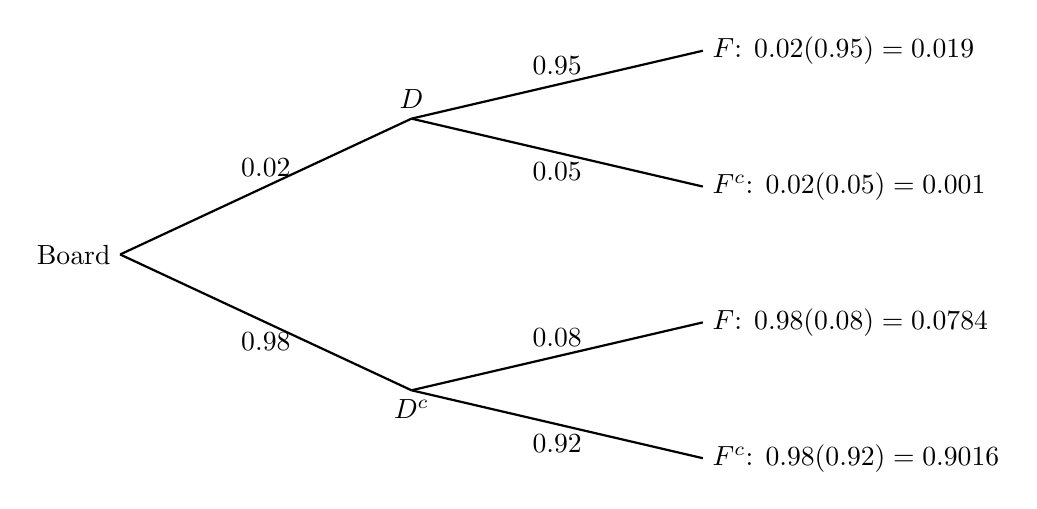
\begin{tikzpicture}[x=3.7cm,y=1.15cm]
  \coordinate (root) at (0,0);
  \coordinate (d) at (1,1.5);
  \coordinate (g) at (1,-1.5);
  \coordinate (df) at (2,2.25);
  \coordinate (dn) at (2,0.75);
  \coordinate (gf) at (2,-0.75);
  \coordinate (gn) at (2,-2.25);
  \draw[thick] (root) -- node[above] {$0.02$} (d);
  \draw[thick] (root) -- node[below] {$0.98$} (g);
  \draw[thick] (d) -- node[above] {$0.95$} (df);
  \draw[thick] (d) -- node[below] {$0.05$} (dn);
  \draw[thick] (g) -- node[above] {$0.08$} (gf);
  \draw[thick] (g) -- node[below] {$0.92$} (gn);
  \node[left] at (root) {Board};
  \node[above] at (d) {$D$};
  \node[below] at (g) {$D^c$};
  \node[right] at (df) {$F$: $0.02(0.95)=0.019$};
  \node[right] at (dn) {$F^c$: $0.02(0.05)=0.001$};
  \node[right] at (gf) {$F$: $0.98(0.08)=0.0784$};
  \node[right] at (gn) {$F^c$: $0.98(0.92)=0.9016$};
\end{tikzpicture}
\caption{Probability tree for the optical inspection system.}
\label{fig:ch2-tree}
\end{figure}

\section{Independence and mutual exclusivity}

\begin{definition}[Independence]
Events $A$ and $B$ are \textbf{independent} if
\[
    P(A\cap B)=P(A)P(B).
\]
When $P(B)>0$, this is equivalent to $P(A\mid B)=P(A)$.
\end{definition}

Independence means that learning whether one event occurred does not change
the probability of the other. It must be supported by the process or model,
not assumed for convenience.

\begin{definition}[Mutually exclusive events]
Events $A$ and $B$ are \textbf{mutually exclusive} if
$A\cap B=\emptyset$.
\end{definition}

If mutually exclusive events both have positive probability, observing one
rules out the other, so they are dependent. For example, $F$ and $F^c$ are
mutually exclusive but not independent when $0<P(F)<1$. Results from
consecutive boards should be modelled as independent only if common machine
drift or batch effects are negligible.

\section{Total probability and Bayes' theorem}

A set of mutually exclusive events whose union is $S$ is a
\textbf{partition}. Events $D$ and $D^c$ partition the board population.

\begin{theorem}[Law of total probability]
If $B_1,\ldots,B_k$ form a partition of $S$, then
\[
    P(A)=\sum_{i=1}^{k}P(A\mid B_i)P(B_i).
\]
\end{theorem}

For the inspection system,
\[
\begin{aligned}
P(F)&=P(F\mid D)P(D)+P(F\mid D^c)P(D^c)\\
&=0.95(0.02)+0.08(0.98)=0.0974.
\end{aligned}
\]

\begin{theorem}[Bayes' theorem]
If $B_1,\ldots,B_k$ form a partition and $P(A)>0$, then
\[
P(B_j\mid A)=
\frac{P(A\mid B_j)P(B_j)}
{\sum_{i=1}^{k}P(A\mid B_i)P(B_i)}.
\]
For a two-part partition,
\[
P(B\mid A)=
\frac{P(A\mid B)P(B)}
{P(A\mid B)P(B)+P(A\mid B^c)P(B^c)}.
\]
\end{theorem}

Bayes' theorem reverses the direction of conditioning. The numerator is the
joint probability of the hypothesis and evidence; the denominator is the
total probability of the evidence across every path.

\section{Worked engineering example}

\[
\begin{aligned}
P(D\mid F)
&=\frac{P(F\mid D)P(D)}
{P(F\mid D)P(D)+P(F\mid D^c)P(D^c)}\\
&=\frac{0.95(0.02)}{0.95(0.02)+0.08(0.98)}
\approx 0.195.
\end{aligned}
\]

A flagged board has a 19.5\% probability of being defective under this model.
About 80.5\% of flags are false positives. This does not contradict the 95\%
sensitivity: 190 of 200 defective boards are caught, but the much larger
group of good boards produces 784 false alarms.

A flag still increases risk from the 2\% base rate to 19.5\%. Whether that is
sufficient to scrap a board depends on the costs of confirmation, missed
defects, and unnecessary scrap. A sensible workflow may send flagged boards
to a more accurate confirmatory test.

The same inspection system produces different predictive values in
populations with different defect rates.

\clearpage
\section{Python in practice}

Figure~\ref{fig:ch2-base-rate} visualises the base-rate effect before we
reproduce the calculation in Python.

\begin{figure}[htbp]
    \centering
    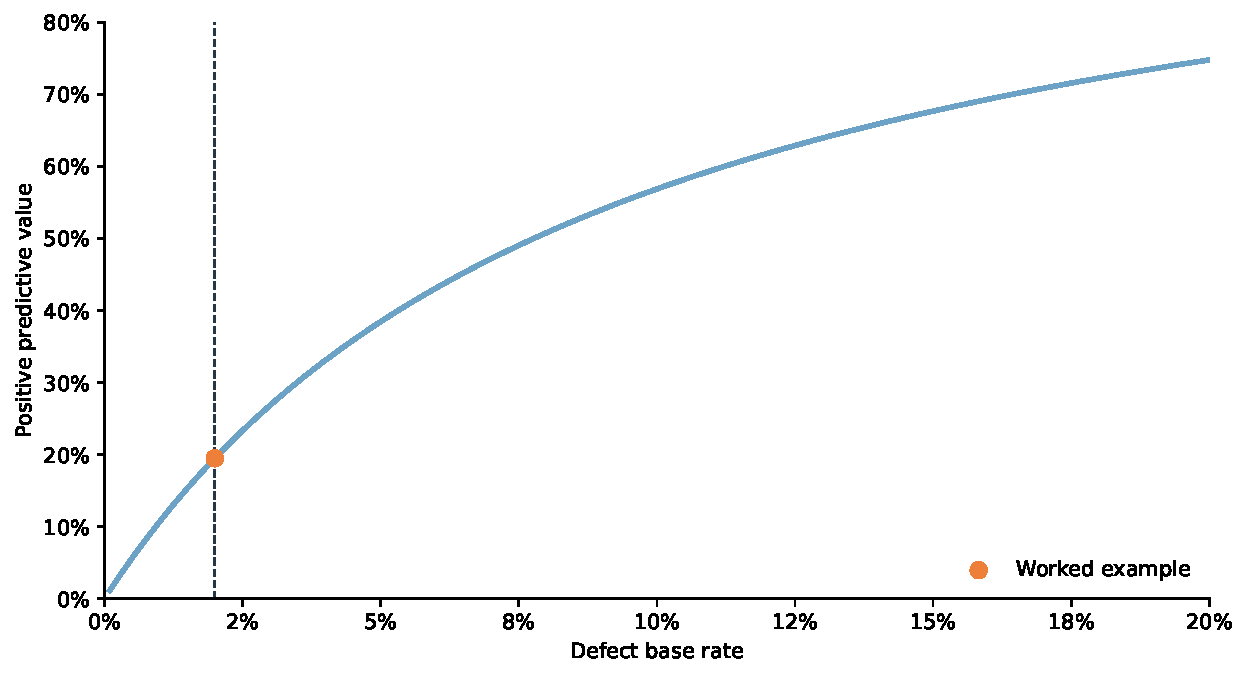
\includegraphics[width=0.88\textwidth]{figure/chapter02_base_rate.pdf}
    \caption{Positive predictive value as a function of defect base rate for
    sensitivity 0.95 and false-positive rate 0.08.}
    \label{fig:ch2-base-rate}
\end{figure}

\begin{python}
import numpy as np
import pandas as pd
import matplotlib.pyplot as plt

p_defect = 0.02
sensitivity = 0.95
false_positive_rate = 0.08

p_flag = (
    sensitivity * p_defect
    + false_positive_rate * (1 - p_defect)
)
ppv = sensitivity * p_defect / p_flag

print(f"P(flag) = {p_flag:.4f}")
print(f"P(defect | flag) = {ppv:.4f}")
\end{python}

Natural frequencies make the denominators visible:

\begin{python}
n = 10_000
n_defective = round(n * p_defect)
n_good = n - n_defective

tp = round(n_defective * sensitivity)
fn = n_defective - tp
fp = round(n_good * false_positive_rate)
tn = n_good - fp

table = pd.DataFrame(
    {"flagged": [tp, fp], "not_flagged": [fn, tn]},
    index=["defective", "good"],
)
table["total"] = table.sum(axis=1)
table.loc["total"] = table.sum(axis=0)
print(table)
\end{python}

Simulation checks the long-run interpretation, but does not replace the exact
calculation:

\begin{python}
rng = np.random.default_rng(2026)
n_sim = 100_000

defective = rng.random(n_sim) < p_defect
flagged = np.where(
    defective,
    rng.random(n_sim) < sensitivity,
    rng.random(n_sim) < false_positive_rate,
)

simulated_ppv = defective[flagged].mean()
print(f"Simulated P(defect | flag) = {simulated_ppv:.4f}")
\end{python}

\begin{quote}
Under a 2\% defect base rate, 95\% sensitivity, and an 8\% false-positive
rate, a flagged board has a 19.5\% probability of being defective. A flag
should trigger confirmation rather than be treated as proof.
\end{quote}

\section{Common pitfalls and chapter summary}

\subsection*{Common pitfalls}
\begin{itemize}
    \item \textbf{Reversing the condition.} $P(F\mid D)$ and $P(D\mid F)$ answer
          different questions.
    \item \textbf{Ignoring the base rate.} Sensitivity alone cannot determine
          positive predictive value.
    \item \textbf{Double-counting a union.} Subtract $P(A\cap B)$ unless the
          events are mutually exclusive.
    \item \textbf{Confusing exclusivity with independence.} Disjoint
          positive-probability events are dependent.
    \item \textbf{Multiplying marginal probabilities automatically.}
          $P(A\cap B)=P(A)P(B)$ requires independence.
    \item \textbf{Treating inputs as timeless facts.} Base rates and error
          rates can change across populations and conditions.
\end{itemize}

\subsection*{Chapter summary}

Events are subsets of a sample space. Complements handle not, intersections
handle and, and unions handle inclusive or. Conditional probability changes
the reference group. Independence means conditioning does not change a
probability; it is not mutual exclusivity. Probability trees and the
multiplication rule construct joint probabilities, total probability adds
mutually exclusive paths, and Bayes' theorem reverses conditioning.

\clearpage
\section{Exercises}

\begin{enumerate}
    \item A server request can succeed, time out, or return an application
    error. Define a sample space and the event that the request fails. Explain
    how the sample space changes if response time is recorded continuously.

    \item Let $P(A)=0.18$, $P(B)=0.25$, and $P(A\cap B)=0.09$ for memory and
    latency warnings. Find $P(A\cup B)$, $P(A-B)$, and the probability of
    neither warning.

    \item A quality sample contains 72 flagged defective items, 8 unflagged
    defective items, 45 flagged good items, and 875 unflagged good items.
    Compute sensitivity, false-positive rate, positive predictive value,
    negative predictive value, and accuracy. Interpret each denominator.

    \item Give one engineering example of mutually exclusive events and one
    of events that could reasonably be independent. Justify both.

    \item A component comes from line A with probability 0.65 and line B with
    probability 0.35. Failure probabilities are 0.01 and 0.04. Draw a tree,
    find the overall failure probability, and find the probability that a
    failed component came from line B.

    \item Reproduce Table~\ref{tab:ch2-confusion} in Pandas and verify the
    three displayed conditional probabilities from its row and column totals.

    \item Reproduce Figure~\ref{fig:ch2-base-rate}. Compare predictive value
    at base rates 0.5\%, 2\%, 10\%, and 20\%. Explain why sensitivity alone is
    insufficient.

    \item Simulate the inspection example for $n=1000$, $10\,000$, and
    $100\,000$ with \texttt{default\_rng(2026)}. Compare with the exact result.

    \item Reduce the false-positive rate from 0.08 to 0.01 while sensitivity
    remains 0.95. Calculate the new predictive value and expected false alarms
    per 10,000 boards.

    \item Correct the claim that a detector with 95\% sensitivity gives every
    flagged board a 95\% probability of being defective.
\end{enumerate}

\chapter{Random Variables and Discrete Distributions}
\label{ch:discrete-distributions}

In \autoref{ch:probability-data-analysis}, probabilities were assigned to events: a component fails, a test returns a positive result, or a system experiences a particular combination of outcomes. In many applications, however, the outcome of interest is numerical. We may want to record the number of failed requests in an hour, the number of defective components in a batch, or the number of attempts required before a transmission succeeds. To analyse such quantities systematically, we introduce the concept of a \textbf{random variable}.

A random variable connects the outcomes of a random experiment with numbers. This allows an uncertain process to be described using familiar mathematical ideas such as functions, sums, averages, and variation. The possible values of the variable do not all need to be equally likely. Their probabilities form a distribution, which provides a complete probabilistic description of the variable and makes it possible to answer questions about both individual outcomes and long-run behaviour.

This chapter focuses on \textbf{discrete random variables}, whose possible values form a finite or countable set. A packet is either lost or delivered; a test suite contains an integer number of failures; and a queue receives a countable number of requests during a specified interval. These examples lead naturally to three important models. The Bernoulli distribution describes a single trial with two possible outcomes. The binomial distribution describes the number of successes in a fixed number of independent Bernoulli trials. The Poisson distribution describes counts occurring within a fixed interval of time, space, or another exposure measure.

Before studying these models, we develop the general language used to describe discrete random variables. Probability mass functions assign probabilities to individual values, while cumulative distribution functions describe probabilities up to a specified threshold. Expected value and variance then summarise the centre and spread of a distribution. Together, these concepts provide the foundation for selecting, interpreting, and applying discrete probability models throughout statistics and data analysis.

\section{Random variables, PMFs, and CDFs}
\label{sec:random-variables-pmf-cdf}

An event describes a collection of outcomes, but it does not necessarily describe them numerically. For example, suppose that two components are inspected and that each component either passes or fails. The sample space may be written as
\[
S=\{PP,PF,FP,FF\},
\]
where $PF$ means that the first component passes and the second fails. If the quantity of interest is the \emph{number} of failed components, the four outcomes are represented by the numbers $0$, $1$, and $2$. A random variable formalises this assignment.

\begin{definition}{Random Variable}
    Let $S$ be the sample space of a random experiment. A \textbf{random variable} is a function
    \[
    X:S\longrightarrow \mathbb{R}
    \]
    that assigns a real number $X(\omega)$ to each outcome $\omega\in S$.
\end{definition}

The word \emph{variable} can be slightly misleading. A random variable is a function with a fixed rule; it is the outcome of the underlying experiment, and therefore the resulting numerical value, that is uncertain. Before the experiment is observed, the random variable is denoted by an uppercase letter such as $X$. A particular realised value is denoted by the corresponding lowercase letter $x$.

\begin{example}[ Number of Failed Components]\par
Let $X$ denote the number of failed components when two components are inspected. The mapping from the sample space to the real numbers is
\[
X(PP)=0,\qquad X(PF)=1,\qquad X(FP)=1,\qquad X(FF)=2.
\]
Notice that different outcomes can produce the same value of $X$. In particular, the event that exactly one component fails is
\[
\{X=1\}=\{PF,FP\}.
\]
Thus, a statement involving a random variable defines an event in the original sample space.
\end{example}

Random variables may be discrete or continuous. A discrete random variable takes values in a finite or countably infinite set. Counts are therefore discrete, even when there is no fixed upper bound. A continuous random variable can take values throughout an interval and will be studied in \autoref{ch:continuous-distributions}.

\begin{definition}{Discrete Random Variable and Support}
    A random variable $X$ is \textbf{discrete} if its possible values form a finite or countably infinite set. The set of values with positive probability is called the \textbf{support} of $X$:
    \[
    \operatorname{supp}(X)=\{x\in\mathbb{R}:P(X=x)>0\}.
    \]
\end{definition}

For the component example, $\operatorname{supp}(X)=\{0,1,2\}$. The support records the possible numerical values, while the probability distribution specifies how probability is allocated among them.

\subsection{The probability mass function}

The distribution of a discrete random variable is described by its probability mass function. It gives the probability of every individual value in the support.

\begin{definition}{Probability Mass Function}
    The \textbf{probability mass function} (PMF) of a discrete random variable $X$ is the function
    \[
    p_X(x)=P(X=x).
    \]
    For values outside the support of $X$, $p_X(x)=0$.
\end{definition}

\clearpage

\begin{theorem}{Properties of a Probability Mass Function}
    A function $p_X$ is a valid PMF if and only if
    \begin{enumerate}
        \item $p_X(x)\geq 0$ for every $x$, and
        \item the probabilities over all values in the support sum to one:
        \[
        \sum_{x\in\operatorname{supp}(X)}p_X(x)=1.
        \]
    \end{enumerate}
    For any set $A\subseteq\mathbb{R}$,
    \[
    P(X\in A)=\sum_{x\in A\cap\operatorname{supp}(X)}p_X(x).
    \]
\end{theorem}

The final formula is particularly important: probabilities involving a discrete random variable are found by adding the probability masses of the values that satisfy the event.

\begin{example}[ PMF for Failed Components]\par
Suppose the two component inspections are independent and that each component fails with probability $0.1$. The probabilities associated with the four outcomes are
\[
\begin{aligned}
P(PP)&=0.9\cdot0.9=0.81,\\
P(PF)&=0.9\cdot0.1=0.09,\\
P(FP)&=0.1\cdot0.9=0.09,\\
P(FF)&=0.1\cdot0.1=0.01.
\end{aligned}
\]
Since $X$ counts the number of failures, its PMF is
\[
\begin{array}{c|ccc}
x & 0 & 1 & 2\\ \hline
p_X(x) & 0.81 & 0.18 & 0.01
\end{array}
\]
where $p_X(1)=P(PF)+P(FP)=0.18$. The values are non-negative and
\[
0.81+0.18+0.01=1,
\]
so the PMF is valid. The probability that at least one component fails is
\[
P(X\geq1)=p_X(1)+p_X(2)=0.18+0.01=0.19.
\]
Equivalently, the complement rule gives $P(X\geq1)=1-p_X(0)=1-0.81=0.19$.
\end{example}

The notation $p_X(x)$ identifies both the random variable and the value being considered. When several random variables occur in the same analysis, the subscript prevents ambiguity. The symbol $p$ without a subscript is often used for a model parameter, so keeping the subscript on a PMF is useful.

\begin{example}[ Determining an Unknown PMF Constant]\par
Suppose a discrete random variable $X$ has support $\{0,1,2,3\}$ and PMF
\[
p_X(x)=c(x+1),\qquad x\in\{0,1,2,3\},
\]
where $c$ is an unknown constant. Since the probability masses must sum to one,
\[
\sum_{x=0}^{3}p_X(x)
=c(1+2+3+4)
=10c
=1.
\]
Therefore, $c=0.1$, and the PMF values are
\[
\begin{array}{c|cccc}
x & 0 & 1 & 2 & 3\\ \hline
p_X(x) & 0.1 & 0.2 & 0.3 & 0.4.
\end{array}
\]
For example,
\[
P(X\geq2)=p_X(2)+p_X(3)=0.3+0.4=0.7.
\]
\end{example}

\subsection{The cumulative distribution function}

A PMF assigns probability to individual values. The cumulative distribution function instead accumulates all probability at or below a threshold. Unlike a PMF, a CDF is defined for every real number and can therefore be used for discrete as well as continuous random variables.

\begin{definition}{Cumulative Distribution Function}
    The \textbf{cumulative distribution function} (CDF) of a random variable $X$ is
    \[
    F_X(x)=P(X\leq x),\qquad x\in\mathbb{R}.
    \]
\end{definition}

For a discrete random variable, the CDF is obtained by summing the probability masses up to $x$:
\[
F_X(x)=\sum_{t\leq x}p_X(t).
\]
The summation includes only values $t$ in the support of $X$. Consequently, the CDF of a discrete random variable is a step function. It remains constant between successive support values and jumps by $p_X(x)$ at each value $x$ in the support.

\begin{theorem}{Properties of a Cumulative Distribution Function}
    Every CDF $F_X$ has the following properties:
    \begin{enumerate}
        \item $0\leq F_X(x)\leq1$ for every $x\in\mathbb{R}$;
        \item $F_X$ is non-decreasing: if $a<b$, then $F_X(a)\leq F_X(b)$;
        \item $F_X$ is right-continuous;
        \item
        \[
        \lim_{x\to-\infty}F_X(x)=0
        \qquad\text{and}\qquad
        \lim_{x\to\infty}F_X(x)=1.
        \]
    \end{enumerate}
\end{theorem}

These properties follow from the interpretation of $F_X(x)$ as accumulated probability. Raising the threshold cannot remove outcomes, and a sufficiently small or sufficiently large threshold eventually includes none or all of the possible values.

\begin{example}[ CDF for Failed Components]\par
For the number of failed components, the PMF values are $0.81$, $0.18$, and $0.01$ at $0$, $1$, and $2$, respectively. Therefore,
\[
F_X(x)=
\begin{cases}
0, & x<0,\\
0.81, & 0\leq x<1,\\
0.99, & 1\leq x<2,\\
1, & x\geq2.
\end{cases}
\]
At $x=1$, for example,
\[
F_X(1)=P(X\leq1)=p_X(0)+p_X(1)=0.81+0.18=0.99.
\]
The CDF jumps by $0.81$ at $0$, by $0.18$ at $1$, and by $0.01$ at $2$. Each jump is exactly the corresponding PMF value.
\end{example}

The CDF is especially convenient for threshold and interval probabilities. For any real numbers $a<b$,
\[
P(a<X\leq b)=F_X(b)-F_X(a).
\]
Tail probabilities follow from the complement rule:
\[
P(X>x)=1-F_X(x).
\]
Care is required with strict and non-strict inequalities for a discrete random variable because an individual value can have positive probability. For an integer-valued random variable,
\[
P(X\geq k)=1-F_X(k-1),
\]
not $1-F_X(k)$.

\begin{example}[ Probabilities from a CDF]\par
Return to the random variable with PMF
\[
p_X(0)=0.1,\qquad p_X(1)=0.2,\qquad p_X(2)=0.3,\qquad p_X(3)=0.4.
\]
Its CDF at the support values is
\[
F_X(0)=0.1,\qquad F_X(1)=0.3,\qquad F_X(2)=0.6,\qquad F_X(3)=1.
\]
The probability that $X$ is strictly greater than $1$ is
\[
P(X>1)=1-F_X(1)=1-0.3=0.7.
\]
The probability that $X$ lies between $1$ and $3$, excluding $1$ but including $3$, is
\[
P(1<X\leq3)=F_X(3)-F_X(1)=1-0.3=0.7.
\]
If the lower endpoint is included instead, then
\[
P(1\leq X\leq3)=1-F_X(0)=1-0.1=0.9.
\]
The difference occurs because $P(X=1)=0.2$.
\end{example}

The PMF and CDF contain the same information for a discrete random variable. The CDF is obtained by accumulating the PMF, and the PMF is recovered from the jumps of the CDF. Writing
\[
F_X(x^-)=\lim_{t\uparrow x}F_X(t)
\]
for the value immediately to the left of $x$, we have
\[
p_X(x)=F_X(x)-F_X(x^-).
\]
For an integer-valued random variable, this becomes
\[
p_X(k)=F_X(k)-F_X(k-1).
\]
The choice between PMF and CDF therefore depends on the question. The PMF is natural for exact values such as $P(X=2)$, whereas the CDF is often more convenient for thresholds, ranges, and tail probabilities.

\section{Expectation and variance}
\label{sec:expectation-variance}

A probability distribution describes all possible values of a random variable and the probability attached to each value. For many purposes, however, it is useful to summarise the distribution using a small number of quantities. The \textbf{expected value} describes its centre, while the \textbf{variance} and \textbf{standard deviation} describe how widely its probability is spread around that centre.

These quantities are properties of a probability model. They should therefore be distinguished from the descriptive measures introduced in \autoref{ch:data-descriptive-statistics}. The expected value $E[X]$ is the theoretical mean of the random variable $X$, whereas a sample mean $\bar{x}$ is calculated from observed data. Similarly, $\operatorname{Var}(X)$ describes variation in the probability distribution, whereas a sample variance $s^2$ is calculated from a particular sample.

\phantomsection
\subsection{Expected value}

Suppose that a discrete random variable $X$ has support $\{x_1,x_2,\ldots\}$. Its expected value is a probability-weighted average of these possible values. Values with high probability contribute more than values with low probability.

\begin{definition}{Expected Value of a Discrete Random Variable}
    Let $X$ be a discrete random variable with PMF $p_X$. The \textbf{expected value}, or \textbf{mean}, of $X$ is
    \[
    E[X]=\sum_{x\in\operatorname{supp}(X)}x\,p_X(x),
    \]
    provided that the sum exists. The expected value is also denoted by $\mu_X$ or simply $\mu$ when the random variable is clear from context.
\end{definition}

The expected value is not necessarily a possible value of the random variable. It describes the long-run average obtained by repeating the random experiment under the same conditions, not the result expected in any one trial.

\begin{example}[ Expected Number of Failed Components]\par
For the number $X$ of failed components introduced in \autoref{sec:random-variables-pmf-cdf}, the PMF is
\[
\begin{array}{c|ccc}
x & 0 & 1 & 2\\ \hline
p_X(x) & 0.81 & 0.18 & 0.01.
\end{array}
\]
The expected number of failed components is therefore
\[
\begin{aligned}
E[X]
&=0\cdot0.81+1\cdot0.18+2\cdot0.01\\
&=0.20.
\end{aligned}
\]
This does not mean that $0.20$ of a component will fail in a particular inspection. It means that over many inspections of two components, the average number of failures per inspection will approach $0.20$ if the model is appropriate. For example, across $1000$ such inspections, the model predicts approximately $1000\cdot0.20=200$ failed components in total.
\end{example}

\begin{example}[ Expected Value of a Fair Die]\par
Let $X$ be the number shown on a fair six-sided die. Since every value has probability $1/6$,
\[
\begin{aligned}
E[X]
&=1\cdot\frac{1}{6}+2\cdot\frac{1}{6}+\cdots+6\cdot\frac{1}{6}\\
&=\frac{1+2+3+4+5+6}{6}\\
&=3.5.
\end{aligned}
\]
No single roll can produce $3.5$. The value is nevertheless the centre of the probability distribution and the long-run average of repeated rolls.
\end{example}

Expected value is linear. Multiplying every possible value by a constant multiplies the expected value by the same constant, and adding a constant shifts the expected value by that amount.

\begin{theorem}{Linearity of Expected Value}
    If $X$ is a random variable with a finite expected value and $a$ and $b$ are constants, then
    \[
    E[aX+b]=aE[X]+b.
    \]
\end{theorem}

More generally, an engineering quantity of interest may be a function of a random variable. If $Y=g(X)$, it is not necessary to determine the complete PMF of $Y$ before calculating its expectation. Each possible value $g(x)$ can be weighted directly by the probability $p_X(x)$.

\begin{theorem}{Expectation of a Function of a Random Variable}
    Let $X$ be a discrete random variable with PMF $p_X$, and let $g$ be a real-valued function. Then
    \[
    E[g(X)]
    =\sum_{x\in\operatorname{supp}(X)}g(x)p_X(x),
    \]
    provided that the sum exists.
\end{theorem}

The linearity result follows by choosing $g(x)=ax+b$. The more general form is useful when costs, energy consumption, response penalties, or other consequences depend nonlinearly on the outcome.

\begin{example}[ Expected Inspection Cost]\par
Suppose that inspecting a pair of components has a fixed setup cost of EUR~$50$, and every failed component produces an additional cost of EUR~$600$. If $X$ is the number of failed components, the total cost is
\[
C=50+600X.
\]
Using linearity and the result $E[X]=0.20$,
\[
E[C]
=50+600E[X]
=50+600\cdot0.20
=170.
\]
Thus, the expected cost is EUR~$170$ per inspection. This is a long-run average cost; an individual inspection costs EUR~$50$, EUR~$650$, or EUR~$1250$ depending on whether zero, one, or two components fail.
\end{example}

\pagebreak
\begin{example}[ Expected Loss under a Nonlinear Penalty]\par
Suppose instead that a simultaneous failure of both components is especially disruptive. Let $L=g(X)$ be the loss, where $g(0)=0$, $g(1)=500$, and $g(2)=5000$, measured in euros.
The expected loss is
\[
\begin{aligned}
E[L]
&=g(0)p_X(0)+g(1)p_X(1)+g(2)p_X(2)\\
&=0\cdot0.81+500\cdot0.18+5000\cdot0.01\\
&=140.
\end{aligned}
\]
Using $g(E[X])$ would not give the correct result: the penalty is nonlinear, and $g(0.20)$ is not even defined by the stated loss table. The probabilities must be applied to the possible losses themselves.
\end{example}

\subsection{Variance and standard deviation}

Two distributions can have the same expected value while assigning probability very differently around it. Expected value alone therefore does not describe the uncertainty in a random variable. Variance measures the expected squared distance from the mean.

\begin{definition}{Variance and Standard Deviation}
    Let $X$ be a random variable with mean $\mu_X=E[X]$. The \textbf{variance} of $X$ is
    \[
    \operatorname{Var}(X)
    =E\big[(X-\mu_X)^2\big].
    \]
    For a discrete random variable,
    \[
    \operatorname{Var}(X)
    =\sum_{x\in\operatorname{supp}(X)}(x-\mu_X)^2p_X(x).
    \]
    The \textbf{standard deviation} of $X$ is
    \[
    \sigma_X=\sqrt{\operatorname{Var}(X)}.
    \]
\end{definition}

The distances from the mean are squared for two reasons. First, positive and negative deviations cannot cancel. Second, large deviations receive greater weight than small deviations. Variance is always non-negative and equals zero only when $X$ is constant with probability one.

Because the deviations are squared, variance has squared units. If $X$ is measured in milliseconds, then $\operatorname{Var}(X)$ is measured in square milliseconds. Standard deviation has the same unit as $X$ and is therefore usually easier to interpret directly.

The definition of variance is conceptually important, but the following equivalent formula is often more convenient for calculation.

\begin{theorem}{Computational Formula for Variance}
    If $E[X^2]$ is finite, then
    \[
    \operatorname{Var}(X)=E[X^2]-\big(E[X]\big)^2.
    \]
\end{theorem}

\clearpage
\begin{example}[ Variance of the Number of Failed Components]\par
For the component model, $E[X]=0.20$. To use the computational formula, first calculate
\[
\begin{aligned}
E[X^2]
&=0^2\cdot0.81+1^2\cdot0.18+2^2\cdot0.01\\
&=0.22.
\end{aligned}
\]
Therefore,
\[
\operatorname{Var}(X)
=E[X^2]-\big(E[X]\big)^2
=0.22-0.20^2
=0.18,
\]
and
\[
\sigma_X=\sqrt{0.18}\approx0.424.
\]
The expected number of failures is $0.20$ per inspection, and the standard deviation is approximately $0.424$ failures.
\end{example}

Variance responds differently from expectation to a linear transformation. Adding a constant shifts every possible value and the mean by the same amount, so it does not change the distances from the mean. Multiplication by $a$ multiplies every distance by $a$ and every squared distance by $a^2$.

\begin{theorem}{Variance under a Linear Transformation}
    If $X$ has finite variance and $a$ and $b$ are constants, then
    \[
    \operatorname{Var}(aX+b)=a^2\operatorname{Var}(X).
    \]
    Consequently,
    \[
    \sigma_{aX+b}=|a|\sigma_X.
    \]
\end{theorem}

\begin{example}[ Variation in Inspection Cost]\par
For the inspection cost $C=50+600X$, the fixed setup cost changes the mean but contributes no variation. Hence,
\[
\begin{aligned}
\operatorname{Var}(C)
&=600^2\operatorname{Var}(X)\\
&=600^2\cdot0.18\\
&=64\,800,
\end{aligned}
\]
measured in square euros. The standard deviation is
\[
\sigma_C=600\sqrt{0.18}\approx254.56\text{ EUR}.
\]
Thus, the model gives an expected cost of EUR~$170$ with a standard deviation of approximately EUR~$255$. The standard deviation is large relative to the expected cost because the usually low cost is accompanied by a small probability of a much larger failure cost.
\end{example}

\subsection{The mean and variance do not determine the distribution}

Expected value and variance provide useful summaries, but they do not replace the PMF or CDF. Even distributions with the same mean and variance can differ in other ways, and distributions with the same mean can have very different levels of uncertainty.

\begin{example}[ Same Mean, Different Variability]\par
Consider two random variables $X$ and $Y$ with PMFs
\[
\begin{array}{c|ccc}
x & 0 & 1 & 2\\ \hline
p_X(x) & 0.25 & 0.50 & 0.25\\
p_Y(x) & 0.50 & 0 & 0.50.
\end{array}
\]
Both variables have expected value one:
\[
E[X]=0\cdot0.25+1\cdot0.50+2\cdot0.25=1
\]
and
\[
E[Y]=0\cdot0.50+1\cdot0+2\cdot0.50=1.
\]
For $X$,
\[
E[X^2]=0^2\cdot0.25+1^2\cdot0.50+2^2\cdot0.25=1.5,
\]
so
\[
\operatorname{Var}(X)=1.5-1^2=0.5.
\]
For $Y$,
\[
E[Y^2]=0^2\cdot0.50+1^2\cdot0+2^2\cdot0.50=2,
\]
so
\[
\operatorname{Var}(Y)=2-1^2=1.
\]
Although the two models have the same expected value, $Y$ never takes the central value $1$ and places all its probability at the two extremes. Its variance is therefore twice as large. A decision based only on the expected value would overlook this difference in uncertainty.
\end{example}

Expectation and variance will be calculated for each of the named distributions in the following sections. Their values help describe and compare the models, but the choice of model must still be based on the underlying random experiment and the complete form of the distribution.

\clearpage
\section{Bernoulli and binomial models}
\label{sec:bernoulli-binomial-models}

Many engineering measurements begin with a binary question. Did a request complete successfully? Was an intrusion attempt blocked? Did the temperature exceed a specified threshold? Was a delivery late? Did a bearing fail, a casting pass inspection, or a structural element satisfy its load requirement? Each question has two possible answers. A \textbf{Bernoulli model} describes one such trial, while a \textbf{binomial model} describes the number of successes in a fixed collection of repeated Bernoulli trials.

The words \emph{success} and \emph{failure} are conventional labels only. A success is the outcome coded as $1$ and may represent an undesirable event such as a defect, packet loss, late delivery, or security alert. What matters is that the event of interest is defined clearly before the probability model is constructed.

\phantomsection
\subsection{Bernoulli trials}

A single trial with two possible outcomes can be represented numerically by assigning the value $1$ to the event of interest and $0$ to its complement. This numerical representation is also called an indicator random variable.

\begin{definition}{Bernoulli Random Variable}
    A random variable $X$ has a \textbf{Bernoulli distribution} with parameter $p$ if
    \[
    P(X=1)=p
    \qquad\text{and}\qquad
    P(X=0)=1-p,
    \]
    where $0\leq p\leq1$. We write
    \[
    X\sim\operatorname{Bernoulli}(p).
    \]
    The value $1$ denotes success and the value $0$ denotes failure.
\end{definition}

The PMF can be written compactly as
\[
p_X(x)=p^x(1-p)^{1-x},
\qquad x\in\{0,1\}.
\]
When $x=1$, this expression equals $p$; when $x=0$, it equals $1-p$. The CDF is
\[
F_X(x)=
\begin{cases}
0, & x<0,\\
1-p, & 0\leq x<1,\\
1, & x\geq1.
\end{cases}
\]

\begin{theorem}{Mean and Variance of a Bernoulli Random Variable}
    If $X\sim\operatorname{Bernoulli}(p)$, then
    \[
    E[X]=p,
    \qquad
    \operatorname{Var}(X)=p(1-p).
    \]
\end{theorem}

The variance is zero when $p=0$ or $p=1$ because the outcome is then certain. It is largest when $p=0.5$, where the two outcomes are equally likely and the uncertainty about a single trial is greatest.

\begin{example}[ Cybersecurity Alert for One Authentication Attempt]\par
Suppose a monitoring rule flags an authentication attempt with probability $0.03$ under a specified operating condition. Let
\[
X=
\begin{cases}
1, & \text{the attempt is flagged},\\
0, & \text{the attempt is not flagged}.
\end{cases}
\]
Then $X\sim\operatorname{Bernoulli}(0.03)$, and
\[
P(X=1)=0.03,
\qquad
P(X=0)=0.97.
\]
Its mean and variance are
\[
E[X]=0.03
\]
and
\[
\operatorname{Var}(X)=0.03(1-0.03)=0.0291.
\]
The expected value $0.03$ is also the long-run proportion of attempts that the model predicts will be flagged. It is not, by itself, the probability that a flagged attempt is genuinely malicious; that would require information about the accuracy of the rule and the prevalence of malicious attempts, as discussed in \autoref{sec:bayes-theorem}.
\end{example}

\subsection{From Bernoulli trials to a binomial count}

Suppose the same type of Bernoulli trial is repeated $n$ times and that $X$ counts the number of successes. A binomial model is appropriate only when the structure of the repeated experiment satisfies specific assumptions.

\begin{definition}{Binomial Experiment}
    A \textbf{binomial experiment} consists of trials satisfying all four conditions:
    \begin{enumerate}
        \item the number of trials $n$ is fixed in advance;
        \item each trial has exactly two outcomes, labelled success and failure;
        \item the probability of success is the same value $p$ on every trial; and
        \item the trials are independent.
    \end{enumerate}
    The random variable of interest is the number of successes among the $n$ trials.
\end{definition}

The assumptions describe the data-generating process, not merely the observed data. Seeing $7$ failures in $100$ tests does not establish a binomial model. We must also have a reason to regard the $100$ tests as a fixed number of independent trials with a common failure probability.

\subsection{The binomial coefficient}

To derive the probability of exactly $k$ successes, first consider one particular ordering. For example, the sequence
\[
SSFSS
\]
contains four successes and one failure. If the trials are independent, the probability of this particular sequence is
\[
p^4(1-p).
\]
Every other sequence with four successes and one failure has the same probability. We therefore need to count how many different sequences contain exactly $k$ successes among $n$ positions.

\clearpage

\begin{definition}{Binomial Coefficient}
    For integers $0\leq k\leq n$, the \textbf{binomial coefficient}
    \[
    \binom{n}{k}
    =\frac{n!}{k!(n-k)!}
    \]
    is the number of ways to choose the $k$ positions occupied by successes among $n$ positions. By convention, $0!=1$.
\end{definition}

\begin{example}[ Placing Two Defects among Five Units]\par
Suppose five units are inspected and exactly two are defective. Once the two positions containing defects have been chosen, the entire defect pattern is determined. The number of possible patterns is
\[
\binom{5}{2}
=\frac{5!}{2!3!}
=10.
\]
If each unit is independently defective with probability $p$, every one of these ten patterns has probability
\[
p^2(1-p)^3.
\]
Consequently, the total probability of exactly two defective units is
\[
10p^2(1-p)^3.
\]
\end{example}

This is the only counting principle needed for the binomial model: $\binom{n}{k}$ counts the possible placements of $k$ successes, while independence gives the probability of each placement.

\subsection{The binomial distribution}

Combining the number of possible placements with the probability of each placement gives the binomial PMF.

\begin{definition}{Binomial Distribution}
    Let $X$ be the number of successes in $n$ independent Bernoulli trials, each with success probability $p$. Then $X$ has a \textbf{binomial distribution}, written
    \[
    X\sim\operatorname{Bin}(n,p),
    \]
    with PMF
    \[
    p_X(k)
    =P(X=k)
    =\binom{n}{k}p^k(1-p)^{n-k},
    \qquad k=0,1,\ldots,n.
    \]
\end{definition}

The four factors in the PMF have distinct meanings:
\[
\underbrace{\binom{n}{k}}_{\text{placements}}
\underbrace{p^k}_{\text{successes}}
\underbrace{(1-p)^{n-k}}_{\text{failures}}.
\]
The support is $\{0,1,\ldots,n\}$. For an integer $k$ in this support, the CDF is
\[
F_X(k)
=P(X\leq k)
=\sum_{j=0}^{k}\binom{n}{j}p^j(1-p)^{n-j}.
\]

\begin{theorem}{Mean and Variance of a Binomial Random Variable}
    If $X\sim\operatorname{Bin}(n,p)$, then
    \[
    E[X]=np,
    \qquad
    \operatorname{Var}(X)=np(1-p),
    \]
    and
    \[
    \sigma_X=\sqrt{np(1-p)}.
    \]
\end{theorem}

The mean has a direct interpretation. Each of the $n$ trials contributes a success with probability $p$, so the expected number of successes is $n$ times $p$. The variance also adds across the independent Bernoulli trials, giving $n$ times the Bernoulli variance $p(1-p)$. Independence is essential for this variance result.

\begin{example}[ Defective Units in a Production Batch]\par
Suppose a production process has a defect probability of $0.03$ for each unit. Twenty units are selected under conditions that make their defect indicators reasonably independent, and $X$ denotes the number of defective units. Under the stated assumptions,
\[
X\sim\operatorname{Bin}(20,0.03).
\]
The probability of exactly one defective unit is
\[
\begin{aligned}
P(X=1)
&=\binom{20}{1}(0.03)^1(0.97)^{19}\\
&\approx0.3364.
\end{aligned}
\]
The expected number and standard deviation are
\[
E[X]=20\cdot0.03=0.60
\]
and
\[
\sigma_X
=\sqrt{20\cdot0.03\cdot0.97}
\approx0.763.
\]
Thus, the model predicts an average of $0.60$ defective units per group of twenty. This does not imply that most inspected groups contain exactly $0.60$ defects, which is not a possible count.
\end{example}

\subsection{Exact, cumulative, and tail probabilities}

The wording of a problem determines whether the PMF, CDF, or complement rule is most convenient. For $X\sim\operatorname{Bin}(n,p)$,
\[
P(X=k)=p_X(k)
\]
is an exact probability,
\[
P(X\leq k)=F_X(k)
\]
is cumulative, and
\[
P(X\geq k)=1-F_X(k-1)
\]
is an upper-tail probability. For integers $a\leq b$,
\[
P(a\leq X\leq b)=F_X(b)-F_X(a-1).
\]
Careful attention to the endpoints prevents the off-by-one errors discussed for general CDFs in \autoref{sec:random-variables-pmf-cdf}.

For realistic values of $n$, $p$, and $\lambda$, exact, cumulative, and tail probabilities are normally evaluated with statistical software such as Python. The formulas remain the foundation of the calculation: they identify the model, translate the engineering event into probability notation, and determine which tail or interval is required. Software evaluates the resulting sums accurately, but it does not select the model or correct an event that has been formulated incorrectly.

\begin{example}[ Packet Loss in a Software System]\par
Suppose a message contains $100$ packets. Under a simplified model, each packet is lost independently with probability $0.01$, and $X$ is the number of packets that must be retransmitted. Then
\[
X\sim\operatorname{Bin}(100,0.01).
\]
The probability that at least one packet must be retransmitted is most easily found using the complement:
\[
\begin{aligned}
P(X\geq1)
&=1-P(X=0)\\
&=1-\binom{100}{0}(0.01)^0(0.99)^{100}\\
&=1-(0.99)^{100}\\
&\approx0.6340.
\end{aligned}
\]
For at least two retransmissions, subtract the probabilities of zero and one:
\[
\begin{aligned}
P(X\geq2)
&=1-P(X=0)-P(X=1)\\
&=1-(0.99)^{100}
-\binom{100}{1}(0.01)(0.99)^{99}\\
&\approx0.2642.
\end{aligned}
\]
The mean and standard deviation are
\[
E[X]=100\cdot0.01=1
\]
and
\[
\sigma_X=\sqrt{100\cdot0.01\cdot0.99}\approx0.995.
\]
Although only one packet is lost on average, the probability of at least one retransmission is approximately $63.4\%$. Expected counts and event probabilities answer different questions.
\end{example}

\begin{example}[ Late Deliveries in a Supply Chain]\par
A supplier schedules $12$ deliveries during a planning period. Suppose each delivery is late with probability $0.08$, independently of the others, and let $X$ be the number of late deliveries. Then
\[
X\sim\operatorname{Bin}(12,0.08).
\]
The probability of at most one late delivery is
\[
\begin{aligned}
P(X\leq1)
&=P(X=0)+P(X=1)\\
&=(0.92)^{12}
+\binom{12}{1}(0.08)(0.92)^{11}\\
&\approx0.7513.
\end{aligned}
\]
The probability of exactly two late deliveries is
\[
\begin{aligned}
P(X=2)
&=\binom{12}{2}(0.08)^2(0.92)^{10}\\
&\approx0.1835.
\end{aligned}
\]
The expected number of late deliveries is
\[
E[X]=12\cdot0.08=0.96.
\]
\par\noindent These calculations are meaningful only if a common delay mechanism, such as the same port closure or severe weather system, does not create substantial dependence among deliveries.
\end{example}

\begin{example}[ Structural Fastener Tests]\par
Twelve structural fasteners are subjected to identical acceptance tests. Suppose each fastener passes with probability $0.98$, independently of the others, and let $X$ be the number that pass. Then
\[
X\sim\operatorname{Bin}(12,0.98).
\]
The probability that all fasteners pass is
\[
P(X=12)=(0.98)^{12}\approx0.7847.
\]
The probability that at least eleven pass is
\[
\begin{aligned}
P(X\geq11)
&=P(X=11)+P(X=12)\\
&=\binom{12}{11}(0.98)^{11}(0.02)+(0.98)^{12}\\
&\approx0.9769.
\end{aligned}
\]
\par\noindent Requiring every fastener to pass is therefore much more stringent than allowing one failure: the corresponding probabilities are approximately $78.5\%$ and $97.7\%$ under this model.
\end{example}

\subsection{Assessing the binomial assumptions}

A binomial calculation can be numerically correct and still be an inappropriate analysis if its assumptions do not match the engineering process. Each assumption should be connected to a feature of the application.

\pagebreak
\begin{example}[ Can Exceedance Days Be Modelled as Binomial?]\par\noindent
An environmental engineer records whether a river exceeds a warning level on each of $30$ consecutive days and proposes the model
\[
X\sim\operatorname{Bin}(30,p),
\]
where $X$ is the number of exceedance days. The number of trials is fixed and every day has two coded outcomes. However, the remaining assumptions require scrutiny.

Exceedances on consecutive days are likely to be dependent because river levels persist and several days may be influenced by the same storm. The probability of exceedance may also vary with season, upstream releases, and soil saturation. Consequently, a binomial model is not justified merely because the response is binary on each day. It may be a rough approximation under stable conditions and weak dependence, but those conditions must be argued rather than assumed.
\end{example}

Dependence also arises through common-cause mechanisms. Fasteners installed in the same concrete pour may share material and installation conditions. Software requests handled by the same failing service instance may fail together. Deliveries routed through the same port may be delayed together. In each case, treating the outcomes as independent usually understates the chance of clusters of failures.

The constant-probability assumption can fail when equipment wears, operators learn, weather changes, or suppliers differ. Sampling without replacement from a small finite lot creates another problem: after a defective item is selected, the composition of the remaining lot changes. For example, drawing ten bearings without replacement from a lot of fifty containing four defective bearings does not produce independent Bernoulli trials with a constant defect probability. A binomial model may sometimes be an adequate approximation when the sampled fraction is small, but it is not the exact model.

The Bernoulli and binomial distributions therefore provide more than formulas. They express a particular structure: one binary trial, or a fixed number of comparable and independent binary trials. In the next section, the focus shifts from a fixed number of trials to events counted over an interval of time, space, area, volume, or another exposure measure.

\clearpage
\section{Poisson models}
\label{sec:poisson-models}

The binomial distribution counts successes among a fixed number of trials. Many engineering counts arise differently. A server may experience an uncertain number of failures during a day, a sheet of material may contain an uncertain number of surface flaws, or a warehouse may receive an uncertain number of urgent orders during an hour. In these situations, the number of opportunities is not naturally fixed in advance. Instead, events are counted within a specified \textbf{exposure}, such as time, distance, area, volume, number of transactions, or operating hours.

The \textbf{Poisson distribution} is a fundamental model for such counts. It is governed by one parameter, $\lambda$, which is the expected number of events in the stated exposure. The exposure is part of the parameter definition: an expected count of two events per hour is not the same model as an expected count of two events per day.

\phantomsection
\subsection{When a Poisson model is plausible}

A Poisson model is often considered when the following features are reasonable approximations:

\begin{enumerate}
    \item $X$ counts identifiable events in a clearly specified exposure;
    \item the average event rate is approximately stable throughout that exposure;
    \item occurrences do not substantially increase or decrease the chance of further occurrences, so clustering and inhibition are limited; and
    \item there is no small fixed upper bound on the count that is central to the problem.
\end{enumerate}

These are modelling conditions, not facts implied by observing count data. A column of non-negative integers is not automatically Poisson distributed. The mechanism producing the counts and the definition of the exposure must support the model.

\begin{definition}{Poisson Distribution}
    A discrete random variable $X$ has a \textbf{Poisson distribution} with parameter $\lambda>0$ if
    \[
    P(X=k)
    =p_X(k)
    =\frac{e^{-\lambda}\lambda^k}{k!},
    \qquad k=0,1,2,\ldots.
    \]
    We write
    \[
    X\sim\operatorname{Pois}(\lambda).
    \]
\end{definition}

Here, $e\approx2.71828$ is the base of the natural logarithm, and $0!=1$. The support is the set of all non-negative integers. Although the mathematical model has no upper bound, very large counts may have extremely small probabilities when $\lambda$ is modest.

The parameter $\lambda$ is both the centre of the distribution and an expected count for one specific exposure. If a system has a stable average rate $r$ events per unit of exposure and the exposure has size $t$, then
\[
\lambda=rt.
\]
The units cancel in the multiplication, but they remain essential to the interpretation. For example,
\[
\left(0.8\ \frac{\text{failures}}{\text{hour}}\right)
(4\ \text{hours})
=3.2\ \text{failures}.
\]
Thus, the appropriate Poisson parameter for four hours is $3.2$, not $0.8$.

\subsection{PMF, CDF, and tail probabilities}

The PMF gives the probability of an exact count. For $X\sim\operatorname{Pois}(\lambda)$,
\[
P(X=k)=\frac{e^{-\lambda}\lambda^k}{k!}.
\]
The CDF is obtained by summing the PMF:
\[
F_X(k)
=P(X\leq k)
=\sum_{j=0}^{k}\frac{e^{-\lambda}\lambda^j}{j!}.
\]
As with the binomial distribution, complements are often the most efficient way to calculate upper-tail probabilities:
\[
P(X\geq k)=1-F_X(k-1).
\]
In particular,
\[
P(X=0)=e^{-\lambda}
\]
and
\[
P(X\geq1)=1-e^{-\lambda}.
\]

\begin{example}[ Software Failures during an Operating Window]\par
A service experiences failures at an average rate of $0.8$ per hour under stable operating conditions. Let $X$ be the number of failures during a four-hour monitoring window. The parameter for this exposure is
\[
\lambda
=\left(0.8\ \frac{\text{failures}}{\text{hour}}\right)
(4\ \text{hours})
=3.2\ \text{failures},
\]
so
\[
X\sim\operatorname{Pois}(3.2).
\]
The probability of no failures is
\[
P(X=0)=e^{-3.2}\approx0.0408.
\]
The probability of at most two failures is
\[
\begin{aligned}
P(X\leq2)
&=P(X=0)+P(X=1)+P(X=2)\\
&=e^{-3.2}\left(1+3.2+\frac{3.2^2}{2!}\right)\\
&\approx0.3799.
\end{aligned}
\]
Therefore,
\[
P(X\geq3)=1-P(X\leq2)\approx0.6201.
\]
Under this model, three or more failures during the four-hour window are more likely than fewer than three. Whether that rate is operationally acceptable is an engineering decision, not a conclusion supplied by the probability model alone.
\end{example}

\subsection{Mean and variance}

The Poisson distribution has the distinctive property that its mean and variance are equal.

\begin{theorem}{Mean and Variance of a Poisson Random Variable}
    If $X\sim\operatorname{Pois}(\lambda)$, then
    \[
    E[X]=\lambda,
    \qquad
    \operatorname{Var}(X)=\lambda,
    \]
    and
    \[
    \sigma_X=\sqrt{\lambda}.
    \]
\end{theorem}

The equality of mean and variance is a property of the theoretical model. It does not mean that the sample mean and sample variance calculated from a finite dataset must be exactly equal. Their relationship can nevertheless be useful when assessing whether a Poisson model is plausible.

\begin{example}[ Surface Flaws in Manufactured Panels]\par
Suppose surface flaws occur at an average rate of $0.4$ per square metre, and a panel has an area of $5$ square metres. If the rate is stable across the surface and flaws occur without substantial clustering, then
\[
\lambda
=\left(0.4\ \frac{\text{flaws}}{\text{m}^2}\right)
(5\ \text{m}^2)
=2\ \text{flaws}.
\]
Let $X$ be the number of flaws on one panel. Then
\[
X\sim\operatorname{Pois}(2).
\]
The probability of exactly three flaws is
\[
\begin{aligned}
P(X=3)
&=\frac{e^{-2}2^3}{3!}\\
&\approx0.1804.
\end{aligned}
\]
The probability of at least one flaw is
\[
P(X\geq1)=1-e^{-2}\approx0.8647.
\]
Finally,
\[
E[X]=2,
\qquad
\sigma_X=\sqrt{2}\approx1.414.
\]
The model therefore predicts two flaws per panel on average, with a standard deviation of approximately $1.41$ flaws.
\end{example}

\subsection{Changing the exposure}

When the rate is constant, changing the exposure changes $\lambda$ proportionally. If the event rate is $r$ per unit and the exposure changes from $t_1$ to $t_2$, then
\[
\lambda_1=rt_1
\qquad\text{and}\qquad
\lambda_2=rt_2.
\]
It is incorrect to reuse a parameter defined for one exposure without rescaling it to the exposure in the probability question.

\begin{example}[ Urgent Orders during Twenty Minutes]\par
A distribution centre receives urgent orders at an average rate of six per hour. Let $X$ be the number received during the next twenty minutes. Since twenty minutes is one third of an hour,
\[
\lambda
=\left(6\ \frac{\text{orders}}{\text{hour}}\right)
\left(\frac{1}{3}\ \text{hour}\right)
=2\ \text{orders}.
\]
Thus, $X\sim\operatorname{Pois}(2)$. The probability of more than four urgent orders is
\[
\begin{aligned}
P(X>4)
&=1-P(X\leq4)\\
&=1-\sum_{k=0}^{4}\frac{e^{-2}2^k}{k!}\\
&\approx0.0527.
\end{aligned}
\]
The probability of more than four arrivals in twenty minutes is therefore approximately $5.3\%$. Using $\lambda=6$ would answer a different question: the number of arrivals in one hour.
\end{example}

\subsection{Poisson approximation to the binomial distribution}

The Poisson distribution can also approximate a binomial distribution when the number of trials is large, the success probability is small, and
\[
\lambda=np
\]
is of moderate size. The approximation replaces
\[
X\sim\operatorname{Bin}(n,p)
\]
with
\[
X\approx\operatorname{Pois}(np).
\]
It is especially useful for rare-event counts when evaluating the binomial PMF directly is inconvenient. The approximation does not remove the binomial assumptions: the underlying trials must still be independent with a common success probability.

\begin{example}[ Rare Security Incidents]\par
Suppose $10\,000$ independent connection attempts each have probability $0.0002$ of producing a particular security incident. If $X$ is the number of incidents, the exact model is
\[
X\sim\operatorname{Bin}(10\,000,0.0002).
\]
Since $n$ is large and $p$ is small, use the Poisson parameter
\[
\lambda=np=10\,000\cdot0.0002=2.
\]
The probability of at least three incidents is approximately
\[
\begin{aligned}
P(X\geq3)
&\approx1-P(Y\leq2),
\qquad Y\sim\operatorname{Pois}(2),\\
&=1-e^{-2}\left(1+2+\frac{2^2}{2!}\right)\\
&\approx0.3233.
\end{aligned}
\]
The exact binomial probability is also $0.3233$ to four decimal places in this case. Such close agreement is not guaranteed when $p$ is larger or when $n$ is small.
\end{example}

\subsection{Assessing the Poisson assumptions}

The mean--variance relationship provides a useful diagnostic. If repeated counts from comparable exposures have a sample variance substantially larger than their sample mean, the data are said to show \textbf{overdispersion} relative to a Poisson model. Possible causes include clustering, unobserved differences between exposures, a changing event rate, or common-cause failures. A sample variance substantially smaller than the sample mean is called \textbf{underdispersion} and may arise from spacing, inhibition, capacity limits, or unusually regular processes.

Neither pattern proves that a Poisson model is wrong, because sample summaries vary from one dataset to another. They identify features that should be investigated using process knowledge, visualisation, and later statistical methods.

\begin{example}[ Annual Flood-Warning Events]\par
Suppose annual counts of flood-warning events over comparable years have a sample mean of $3.5$ and a sample variance of $9.1$. A Poisson model with $\lambda=3.5$ would have theoretical variance $3.5$, considerably smaller than the observed sample variance.

The difference suggests overdispersion. A plausible explanation is that some years are much wetter than others and that several warnings may arise from the same persistent weather system. The annual rate is then not stable across years, and events within a year may be clustered. The comparison is a diagnostic rather than a formal rejection of the model, but it gives a clear reason to examine the mechanism before using Poisson tail probabilities for planning.
\end{example}

A Poisson model is also inappropriate when the count has a small fixed maximum that matters. The number of failed components among twenty tested components cannot exceed twenty and naturally begins with a binomial model. By contrast, the number of failures during a period of operation may have no comparable fixed trial count and can be a plausible Poisson quantity. The model choice follows from the event-generating structure, not simply from whether the observed variable is a count.

Together, the Bernoulli, binomial, and Poisson distributions cover three common engineering structures: one binary outcome, successes among a fixed number of trials, and events within a specified exposure. Selecting among them requires both a correctly calculated probability and a credible account of how the data are generated.

The models in this chapter describe binary outcomes and event counts. Many engineering quantities, however, are measured on a continuous scale, including response times, dimensions, temperatures, and component lifetimes. The next chapter develops probability models for such continuous measurements.

\chapter{Continuous Distributions in Practice}
\label{ch:continuous-distributions}

Many engineering quantities are measured on a continuous scale. Response times are recorded in milliseconds, component dimensions in millimetres, temperatures in degrees, and lifetimes in hours or cycles. Although an instrument reports a finite number of digits, the underlying quantity is usually modelled as capable of taking any value in an interval. Continuous probability models provide a mathematical description of the uncertainty in such measurements.

This setting differs fundamentally from the discrete models developed in the previous chapter. A discrete random variable assigns probability to individual values through a probability mass function. For a continuous random variable, probabilities are assigned to intervals instead. The probability of observing any one exact value is zero, even though intervals containing that value can have positive probability. A probability density describes how probability is distributed locally, while the cumulative distribution function records the probability of falling below a threshold.

The chapter develops three continuous models that occur frequently in engineering. The uniform distribution represents uncertainty spread evenly across a bounded interval. The normal distribution describes symmetric variation around a central value and is widely used for measurement error and stable process variation. The exponential distribution describes waiting times and lifetimes under a constant event-rate model, providing a direct connection with the Poisson counts introduced previously. Each distribution is an idealised model whose usefulness depends on the mechanism that generated the data and on whether its assumptions are credible.

We first introduce densities, distribution functions, survival probabilities, and quantiles. We then study the uniform, normal, and exponential distributions, including standardisation and interval calculations. Finally, we consider how graphical evidence, especially quantile--quantile plots, can be used to assess whether a proposed model is a reasonable approximation. The emphasis throughout is on interpretation and model choice rather than on manual integration.

\section{Continuous Random Variables, Densities, and Distribution Functions}
\label{sec:continuous-foundations}

A count changes in separate steps: a system can receive 12 or 13 requests, but not 12.4 requests. A measurement behaves differently. Between two possible response times there is, at least conceptually, another possible response time. This distinction motivates a different way of assigning probability.

\subsection{Continuous random variables and support}

\begin{definition}{Continuous Random Variable}
A random variable $X$ is \textbf{continuous} if its probabilities can be described by a probability density function over intervals of real numbers. The set of values on which the density is positive is called the \textbf{support} of the distribution.
\end{definition}

The support may be bounded, such as the interval from 0 to 10 volts, or unbounded, such as all positive waiting times. It may also be the complete real line, as in the normal distribution. The support is part of the model and should agree with the possible values of the engineering quantity.

Recorded data can look discrete even when the underlying model is continuous. A temperature sensor that reports to the nearest $0.1\,^{\circ}\mathrm{C}$ produces values such as $18.3$ and $18.4$, but the physical temperature is not assumed to jump between those values. The rounding belongs to the measurement system; the continuous model describes the underlying quantity.

\begin{example}[ Measurement Resolution and a Continuous Model]\par
A laser scanner reports the thickness of a steel plate to the nearest $0.01$ mm. A displayed value of $12.37$ mm represents a range of underlying thicknesses that round to that number. It does not mean that the true thickness can take only multiples of $0.01$ mm. Modelling the underlying thickness as continuous is therefore compatible with the rounded observations.
\end{example}

\subsection{Probability density functions}

For a discrete random variable, the height of the PMF at $x$ is the probability $P(X=x)$. For a continuous random variable, the height of a density is not a probability. Probability is represented by area under the density over an interval.

\begin{definition}{Probability Density Function}
A function $f_X$ is a \textbf{probability density function} (PDF) for a continuous random variable $X$ if
\[
    f_X(x)\geq 0
\]
for all $x$, the total area under the density is 1,
\[
    \int_{-\infty}^{\infty} f_X(x)\,dx=1,
\]
and
\[
    P(a<X\leq b)=\int_a^b f_X(x)\,dx
\]
for any $a<b$.
\end{definition}

The integral notation expresses an area. In this book, standard distributions supply the relevant areas through their distribution functions; manual integration is not required. The notation remains important because it explains what a density means.

The units of a density are the reciprocal of the units of the random variable. If $X$ is measured in hours, then $f_X(x)$ has units of probability per hour. This is another reason why a density height cannot itself be interpreted as a probability.

\begin{theorem}{Basic Properties of a Continuous Distribution}
If $X$ is continuous, then
\[
    P(X=x)=0
\]
for every exact value $x$. Consequently, for $a<b$,
\[
\begin{aligned}
P(a<X<b)
  &=P(a\leq X<b)\\
  &=P(a<X\leq b)\\
  &=P(a\leq X\leq b).
\end{aligned}
\]
The choice of strict or inclusive endpoints does not change an interval probability.
\end{theorem}

The statement $P(X=x)=0$ does not mean that observing $x$ is impossible. It means that a single point has no area. Every realised measurement is an individual value, but probability calculations concern intervals of possible values.

\begin{figure}[htbp]
\centering
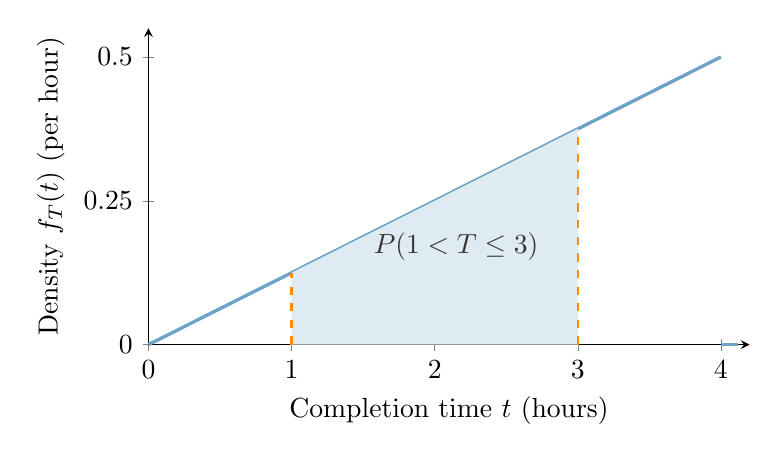
\begin{tikzpicture}
\begin{axis}[
    width=0.76\textwidth,
    height=5.6cm,
    xmin=0,xmax=4.2,
    ymin=0,ymax=0.55,
    axis lines=left,
    xlabel={Completion time $t$ (hours)},
    ylabel={Density $f_T(t)$ (per hour)},
    xtick={0,1,2,3,4},
    ytick={0,0.25,0.5},
    clip=false
]
\addplot[very thick,staViaBlue,domain=0:4,samples=100] {x/8};
\addplot[very thick,staViaBlue,domain=4:4.12] {0};
\addplot[fill=staViaBlue!22,draw=none,domain=1:3,samples=80] {x/8} \closedcycle;
\draw[dashed,staOrange,thick] (axis cs:1,0) -- (axis cs:1,0.125);
\draw[dashed,staOrange,thick] (axis cs:3,0) -- (axis cs:3,0.375);
\node[staDarkText] at (axis cs:2.15,0.17) {$P(1<T\leq3)$};
\end{axis}
\end{tikzpicture}
\caption{For a continuous variable, the shaded area over an interval represents probability. The height of the density at one point is not a probability.}
\label{fig:continuous-density-area}
\end{figure}

\subsection{The cumulative distribution function}

The cumulative distribution function was introduced in \hyperref[sec:random-variables-pmf-cdf]{Section 3.1} for random variables in general. For a continuous variable it accumulates area under the density from the far left up to a threshold.

\begin{definition}{Cumulative Distribution Function for a Continuous Variable}
The \textbf{cumulative distribution function} (CDF) of a continuous random variable $X$ is
\[
    F_X(x)=P(X\leq x).
\]
It is related to the density by
\[
    F_X(x)=\int_{-\infty}^{x} f_X(t)\,dt.
\]
\end{definition}

The letter $t$ inside the integral is a temporary variable. The argument $x$ remains the threshold at which the CDF is evaluated. A continuous CDF is non-decreasing, takes values between 0 and 1, approaches 0 far to the left, and approaches 1 far to the right.

\begin{theorem}{Probabilities from a Continuous CDF}
For a continuous random variable $X$ with CDF $F_X$,
\[
\begin{aligned}
P(X\leq x)&=F_X(x),\\
P(X>x)&=1-F_X(x),\\
P(a<X\leq b)&=F_X(b)-F_X(a).
\end{aligned}
\]
\end{theorem}

These identities are the main computational tools for continuous models. They translate the position of an interval into accumulated probability without requiring direct evaluation of an area.

\begin{example}[ Completion Time from a CDF]\label{ex:completion-time-cdf}\par
Let $T$ be the time, in hours, required to complete a maintenance task. Suppose
\[
F_T(t)=
\begin{cases}
0, & t<0,\\
t^2/16, & 0\leq t\leq4,\\
1, & t>4.
\end{cases}
\]
The probability of completing the task within one hour is
\[
    P(T\leq1)=F_T(1)=\frac{1}{16}=0.0625.
\]
The probability that the task takes more than two hours is
\[
    P(T>2)=1-F_T(2)=1-\frac{4}{16}=0.75.
\]
Finally,
\[
\begin{aligned}
P(1<T\leq3)
  &=F_T(3)-F_T(1)\\
  &=\frac{9}{16}-\frac{1}{16}\\
  &=0.50.
\end{aligned}
\]
Thus half of all such tasks are expected to take between one and three hours under this model. The corresponding density and interval area are illustrated in \autoref{fig:continuous-density-area}.
\end{example}

\subsection{Survival functions and quantiles}

Many engineering questions concern exceeding a threshold: a component surviving beyond 500 hours, a response taking longer than 100 ms, or a river level exceeding a warning limit. Such questions can be written compactly using a survival function.

\begin{definition}{Survival Function}
For a continuous random variable $X$, the \textbf{survival function} is
\[
    S_X(x)=P(X>x)=1-F_X(x).
\]
\end{definition}

The word survival is especially natural for lifetime data, but the function applies to any upper-tail probability. It is often preferable to writing $1-F_X(x)$ repeatedly.

A probability calculation starts from a value and finds an area. A quantile calculation reverses the direction: it starts from an accumulated probability and finds the corresponding value.

\begin{definition}{Quantile}
For $0<p<1$, a \textbf{$p$-quantile} of a continuous distribution is a value $q_p$ satisfying
\[
    F_X(q_p)=p.
\]
When the CDF is strictly increasing, the quantile is unique and can be written
\[
    q_p=F_X^{-1}(p).
\]
The median is the $0.5$-quantile, and the $100p$th percentile is $q_p$.
\end{definition}

\begin{example}[ A Service-Time Guarantee]\par
For the maintenance-time model in \autoref{ex:completion-time-cdf}, suppose a planner wants a time limit that is sufficient for 90\% of tasks. The required value is the $0.9$-quantile. Within the support,
\[
    F_T(t)=\frac{t^2}{16}.
\]
Setting this equal to $0.9$ gives
\[
    \frac{q_{0.9}^2}{16}=0.9,
    \qquad
    q_{0.9}=4\sqrt{0.9}\approx3.79\text{ hours}.
\]
A planning allowance of approximately 3.79 hours is therefore exceeded by 10\% of tasks under the model.
\end{example}

Expected value and variance retain the interpretations developed for discrete random variables: they describe the centre and spread of a distribution. For the named continuous models in this chapter, their values are stated as model properties and interpreted in context. Their calculus-based derivations are not needed here.

\section{The Uniform Distribution}
\label{sec:uniform-distribution}

The uniform distribution is the simplest continuous model. It describes a quantity restricted to a finite interval when equal-length subintervals are assigned equal probability. The density is constant, so probability depends only on interval length.

\begin{definition}{Continuous Uniform Distribution}
A random variable $X$ has a \textbf{continuous uniform distribution} on the interval $[a,b]$, where $a<b$, if its density is
\[
f_X(x)=
\begin{cases}
\dfrac{1}{b-a}, & a\leq x\leq b,\\
0, & \text{otherwise}.
\end{cases}
\]
We write
\[
    X\sim U(a,b).
\]
Its CDF is
\[
F_X(x)=
\begin{cases}
0, & x<a,\\
\dfrac{x-a}{b-a}, & a\leq x\leq b,\\
1, & x>b.
\end{cases}
\]
\end{definition}

\begin{figure}[htbp]
\centering
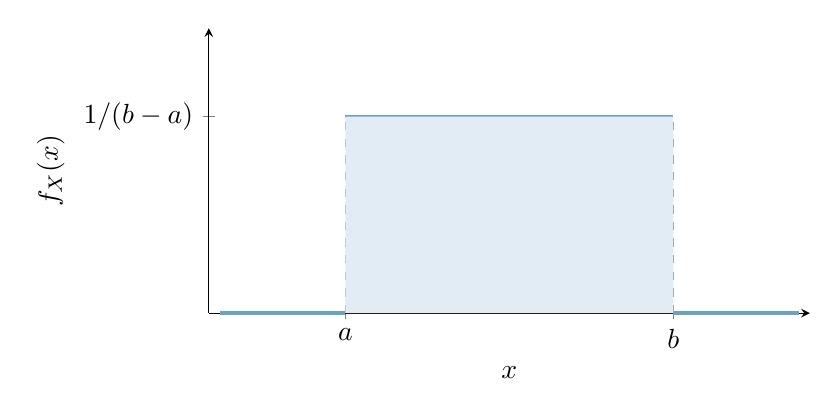
\begin{tikzpicture}
\begin{axis}[
    width=0.76\textwidth,
    height=5.2cm,
    xmin=-0.5,xmax=10.5,
    ymin=0,ymax=0.145,
    axis lines=left,
    xlabel={$x$},
    ylabel={$f_X(x)$},
    xtick={2,8},
    xticklabels={$a$,$b$},
    ytick={0.1},
    yticklabels={$1/(b-a)$},
    clip=false
]
\addplot[very thick,staViaBlue] coordinates {(-0.3,0) (2,0)};
\addplot[very thick,staViaBlue] coordinates {(2,0.1) (8,0.1)};
\addplot[very thick,staViaBlue] coordinates {(8,0) (10.3,0)};
\draw[dashed,staDarkText!60] (axis cs:2,0) -- (axis cs:2,0.1);
\draw[dashed,staDarkText!60] (axis cs:8,0) -- (axis cs:8,0.1);
\addplot[fill=staViaBlue!20,draw=none] coordinates {(2,0) (2,0.1) (8,0.1) (8,0)} \closedcycle;
\end{axis}
\end{tikzpicture}
\caption{The uniform density is constant on $[a,b]$. Its rectangular area is height $1/(b-a)$ times width $b-a$, giving total probability 1.}
\label{fig:uniform-density}
\end{figure}

For any subinterval $[c,d]\subseteq[a,b]$,
\[
    P(c\leq X\leq d)=\frac{d-c}{b-a}.
\]
The formula compares the length of the favourable interval with the length of the complete support. This geometric interpretation is visible in \autoref{fig:uniform-density}.

\begin{theorem}{Mean, Variance, and Quantiles of a Uniform Variable}
If $X\sim U(a,b)$, then
\[
    E[X]=\frac{a+b}{2},
    \qquad
    \operatorname{Var}(X)=\frac{(b-a)^2}{12},
\]
and
\[
    q_p=a+p(b-a), \qquad 0<p<1.
\]
\end{theorem}

The mean is the midpoint of the support. The standard deviation depends only on the width $b-a$: shifting both endpoints by the same amount shifts the mean but leaves the variability unchanged.

\begin{example}[ Delivery within a Scheduled Window]\par
A supplier commits to deliver a specialised component between 18 and 30 days after an order. Suppose that, within this interval, no delivery time is considered more likely than another. Let
\[
    X\sim U(18,30).
\]
The probability of delivery between day 22 and day 25 is
\[
    P(22\leq X\leq25)=\frac{25-22}{30-18}=\frac{3}{12}=0.25.
\]
Similarly,
\[
    P(X>27)=\frac{30-27}{12}=0.25.
\]
The mean and standard deviation are
\[
    E[X]=\frac{18+30}{2}=24\text{ days}
\]
and
\[
    \sqrt{\operatorname{Var}(X)}
      =\sqrt{\frac{(30-18)^2}{12}}
      =\sqrt{12}
      \approx3.46\text{ days}.
\]
The 90th percentile is
\[
    q_{0.9}=18+0.9(30-18)=28.8\text{ days}.
\]
Thus 90\% of deliveries occur by day 28.8 under the uniform model.
\end{example}

\begin{example}[ Bounded Calibration Error]\par
Suppose the rounding error $E$ of a digital measurement is modelled as uniform between $-0.05$ and $0.05$ units. Then
\[
    E\sim U(-0.05,0.05).
\]
The probability that the absolute error is no more than $0.02$ is
\[
\begin{aligned}
P(|E|\leq0.02)
  &=P(-0.02\leq E\leq0.02)\\
  &=\frac{0.02-(-0.02)}{0.05-(-0.05)}\\
  &=0.40.
\end{aligned}
\]
The model is centred at zero, but only 40\% of its probability lies within $0.02$ units of zero.
\end{example}

\subsection{When is a uniform model reasonable?}

A uniform model requires more than known minimum and maximum values. It asserts that intervals of equal length are equally likely throughout the support. This may be plausible for a deliberately randomised start time, an unknown phase in a repeating cycle, or rounding error under suitable conditions. It is usually not plausible for manufacturing measurements that cluster around a target or for waiting times concentrated near zero.

The bounded support is also a firm assumption: the model assigns zero probability outside $[a,b]$. If values beyond the stated limits can occur, even rarely, the uniform distribution is not an adequate model for the complete process.

\section{The Normal Distribution}
\label{sec:normal-distribution}

The normal distribution is central to statistics because many stable measurement processes produce approximately symmetric, bell-shaped variation. It also arises as an approximation to sums and averages of many small contributions, a connection developed formally in \hyperref[ch:sampling-distributions]{Chapter 5}. Normality is nevertheless a modelling assumption, not a default property of every continuous dataset.

\begin{definition}{Normal Distribution}
A random variable $X$ has a \textbf{normal distribution} with mean $\mu$ and variance $\sigma^2$, where $\sigma>0$, if its density is
\[
    f_X(x)=\frac{1}{\sigma\sqrt{2\pi}}
    \exp\!\left[-\frac{(x-\mu)^2}{2\sigma^2}\right],
    \qquad -\infty<x<\infty.
\]
We write
\[
    X\sim N(\mu,\sigma^2).
\]
\end{definition}

The first parameter is the mean and the second is the variance. The standard deviation is therefore $\sigma$, not $\sigma^2$. The parameter $\mu$ determines the centre of the curve, while $\sigma$ determines its horizontal spread.

\begin{theorem}{Properties of a Normal Distribution}
If $X\sim N(\mu,\sigma^2)$, then
\[
    E[X]=\mu,
    \qquad
    \operatorname{Var}(X)=\sigma^2.
\]
The density is symmetric about $\mu$, so
\[
    P(X\leq\mu)=P(X\geq\mu)=0.5.
\]
Its mean, median, and mode are all equal to $\mu$.
\end{theorem}

\begin{figure}[htbp]
\centering
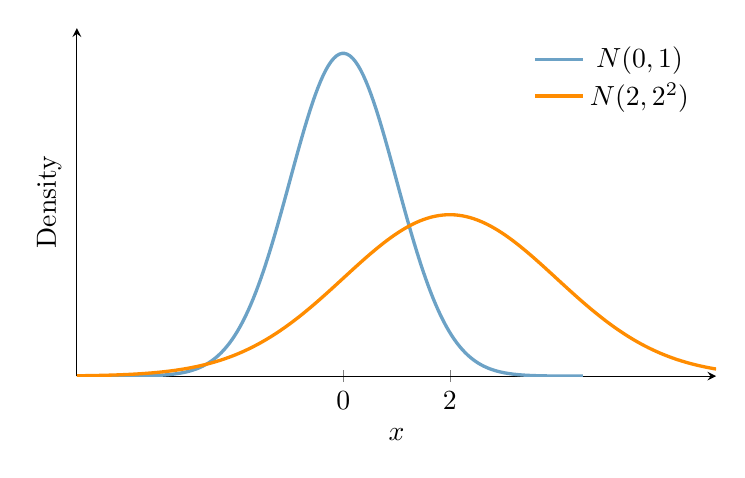
\begin{tikzpicture}
\begin{axis}[
    width=0.80\textwidth,
    height=6.0cm,
    xmin=-5,xmax=7,
    ymin=0,ymax=0.43,
    axis lines=left,
    xlabel={$x$},
    ylabel={Density},
    xtick={0,2},
    xticklabels={$0$,$2$},
    ytick=\empty,
    legend style={draw=none,fill=none,at={(0.98,0.98)},anchor=north east}
]
\addplot[very thick,staViaBlue,domain=-4.5:4.5,samples=180] {1/sqrt(2*pi)*exp(-x^2/2)};
\addlegendentry{$N(0,1)$}
\addplot[very thick,staOrange,domain=-5:7,samples=180] {1/(2*sqrt(2*pi))*exp(-(x-2)^2/8)};
\addlegendentry{$N(2,2^2)$}
\end{axis}
\end{tikzpicture}
\caption{The mean determines the centre of a normal curve and the standard deviation determines its spread. Every normal density is symmetric and has total area 1.}
\label{fig:normal-location-scale}
\end{figure}

Although the normal support is the complete real line, values far from the mean have very small probability. A normal model may therefore be useful for a positive quantity when the mean is many standard deviations above zero. It is inappropriate when the model assigns non-negligible probability to impossible values or when the data are strongly skewed.

\subsection{The standard normal distribution}

All normal distributions can be related to one reference distribution.

\begin{definition}{Standard Normal Distribution}
A normal random variable with mean 0 and variance 1 is called a \textbf{standard normal random variable}. It is denoted by
\[
    Z\sim N(0,1).
\]
Its CDF is written
\[
    \Phi(z)=P(Z\leq z).
\]
\end{definition}

There is no elementary closed formula for $\Phi(z)$. Its values are obtained from numerical evaluation or a standard normal table. Symmetry gives the useful identity
\[
    \Phi(-z)=1-\Phi(z).
\]

\subsection{Using a standard normal table}

A standard normal table gives cumulative left-tail probabilities $\Phi(z)=P(Z\leq z)$. In the common layout illustrated by \autoref{tab:standard-normal-excerpt}, the row supplies the units and first decimal place of $z$, while the column supplies the second decimal place. For example, $z=1.25$ is found in row $1.2$ and column $0.05$, giving
\[
    \Phi(1.25)=0.8944.
\]

\begin{table}[htbp]
\centering
\caption{Excerpt from a cumulative standard normal table. Each entry is $\Phi(z)=P(Z\leq z)$.}
\label{tab:standard-normal-excerpt}
\small
\setlength{\tabcolsep}{3.2pt}
\renewcommand{\arraystretch}{1.15}
\begin{tabular}{@{}c*{10}{c}@{}}
\toprule
$z$ & $0.00$ & $0.01$ & $0.02$ & $0.03$ & $0.04$ & $0.05$ & $0.06$ & $0.07$ & $0.08$ & $0.09$ \\
\midrule
$1.2$ & $0.8849$ & $0.8869$ & $0.8888$ & $0.8907$ & $0.8925$ & $0.8944$ & $0.8962$ & $0.8980$ & $0.8997$ & $0.9015$ \\
$1.5$ & $0.9332$ & $0.9345$ & $0.9357$ & $0.9370$ & $0.9382$ & $0.9394$ & $0.9406$ & $0.9418$ & $0.9429$ & $0.9441$ \\
$1.9$ & $0.9713$ & $0.9719$ & $0.9726$ & $0.9732$ & $0.9738$ & $0.9744$ & $0.9750$ & $0.9756$ & $0.9761$ & $0.9767$ \\
\bottomrule
\end{tabular}
\end{table}

Tables often list only nonnegative $z$-scores. Negative values are then handled by symmetry. For example,
\[
    \Phi(-1.50)=1-\Phi(1.50)=1-0.9332=0.0668.
\]
Right-tail probabilities are found by complementation, and interval probabilities are found by subtracting two cumulative probabilities. The same table can be read in reverse to locate quantiles. An entry of $0.9750$, for instance, occurs at row $1.9$ and column $0.06$, so $z_{0.975}\approx1.96$.

In practical analysis, statistical software such as Python is normally used to evaluate normal probabilities and quantiles. The table remains useful because it makes the direction of a probability calculation visible: the entry is a left-tail probability, while right tails and intervals still require the complement or subtraction rules. Software performs the numerical evaluation; the analyst must still standardise correctly and identify the intended event.

\begin{theorem}{Standardisation of a Normal Variable}
If $X\sim N(\mu,\sigma^2)$, then
\[
    Z=\frac{X-\mu}{\sigma}\sim N(0,1).
\]
\end{theorem}

Consequently,
\[
    P(X\leq x)=
    \Phi\!\left(\frac{x-\mu}{\sigma}\right).
\]

The standardised value
\[
    z=\frac{x-\mu}{\sigma}
\]
is called a \textbf{$z$-score}. It describes how many standard deviations $x$ lies above or below the mean. A positive $z$-score is above the mean, and a negative $z$-score is below it.

\begin{example}[ Shaft Diameter within an Interval]\par
The diameter $X$ of a machined shaft is modelled as
\[
    X\sim N(20.00,0.04^2)\text{ mm}.
\]
The probability that a shaft diameter is between $19.94$ mm and $20.05$ mm is found by standardising both limits:
\[
    z_{\mathrm{lower}}=\frac{19.94-20.00}{0.04}=-1.50,
    \qquad
    z_{\mathrm{upper}}=\frac{20.05-20.00}{0.04}=1.25.
\]
Therefore,
\[
\begin{aligned}
P(19.94\leq X\leq20.05)
  &=\Phi(1.25)-\Phi(-1.50)\\
  &\approx0.8944-0.0668\\
  &=0.8276.
\end{aligned}
\]
Approximately 82.8\% of shafts lie in this interval if the normal model and its parameters are appropriate.
\end{example}

\subsection{Normal quantiles and percentiles}

Let $z_p$ denote the $p$-quantile of the standard normal distribution, so that
\[
    \Phi(z_p)=p.
\]
If $X\sim N(\mu,\sigma^2)$, its $p$-quantile is
\[
    q_p=\mu+z_p\sigma.
\]
This formula converts a standard normal percentile to the original measurement scale.

\begin{example}[ A High Measurement-Error Threshold]\par
The output of a voltage reference is modelled as
\[
    X\sim N(5.00,0.02^2)\text{ V}.
\]
The 99th standard normal percentile is $z_{0.99}\approx2.326$. Hence
\[
\begin{aligned}
q_{0.99}
  &=5.00+2.326(0.02)\\
  &\approx5.0465\text{ V}.
\end{aligned}
\]
Under the model, 99\% of outputs are at or below approximately $5.0465$ V, and 1\% exceed that value.
\end{example}

\subsection{The empirical rule}

The standard normal CDF gives three useful reference probabilities:
\[
\begin{aligned}
P(\mu-\sigma\leq X\leq\mu+\sigma)&\approx0.6827,\\
P(\mu-2\sigma\leq X\leq\mu+2\sigma)&\approx0.9545,\\
P(\mu-3\sigma\leq X\leq\mu+3\sigma)&\approx0.9973.
\end{aligned}
\]
These are often remembered as the \textbf{68--95--99.7 rule}. The rule applies to a normal distribution, not to an arbitrary dataset merely because its mean and standard deviation are known.

\begin{example}[ Process Yield within Symmetric Tolerances]\par
Return to the shaft model $X\sim N(20.00,0.04^2)$ mm. Suppose the acceptable diameter is from $19.92$ mm to $20.08$ mm. These limits are two standard deviations from the mean:
\[
    \frac{19.92-20.00}{0.04}=-2,
    \qquad
    \frac{20.08-20.00}{0.04}=2.
\]
Thus
\[
    P(19.92\leq X\leq20.08)\approx0.9545.
\]
The model predicts a yield of approximately 95.45\% before considering any other defect mechanism. The remaining 4.55\% is split equally between the two tails because the process is centred at the midpoint of the tolerance interval.
\end{example}

\subsection{When is a normal model reasonable?}

A normal model is most plausible when variation is approximately symmetric around a stable centre and results from many small contributions rather than one dominant mechanism. Measurement error, controlled process dimensions, and aggregated environmental variation can sometimes have this form.

The model should be questioned when observations are strongly skewed, bounded close to the centre, contain several distinct clusters, or include more extreme values than a normal distribution would predict. Waiting times and response times are often right-skewed and nonnegative; a raw normal model can then be misleading even if it is convenient. Graphical diagnostics are discussed in \autoref{sec:model-assessment-continuous}.

\section{The Exponential Distribution}
\label{sec:exponential-distribution}

The exponential distribution models the time until an event when events occur at a constant rate and independently of how long one has already waited. Examples include the time until the next request under a stable arrival mechanism or the operating time until a sudden failure under a constant failure-rate model.

\begin{definition}{Exponential Distribution}
A nonnegative random variable $T$ has an \textbf{exponential distribution} with rate $\lambda>0$ if its density is
\[
f_T(t)=
\begin{cases}
\lambda e^{-\lambda t}, & t\geq0,\\
0, & t<0.
\end{cases}
\]
We write
\[
    T\sim\operatorname{Exp}(\lambda).
\]
Its CDF and survival function are
\[
F_T(t)=
\begin{cases}
0, & t<0,\\
1-e^{-\lambda t}, & t\geq0,
\end{cases}
\]
and
\[
    S_T(t)=P(T>t)=e^{-\lambda t}, \qquad t\geq0.
\]
\end{definition}

The parameter $\lambda$ is a rate and therefore has reciprocal time units. If $t$ is measured in hours, then $\lambda$ is measured in events per hour. A larger rate produces shorter waiting times and a density that decreases more rapidly, as shown in \autoref{fig:exponential-densities}.

\begin{figure}[htbp]
\centering
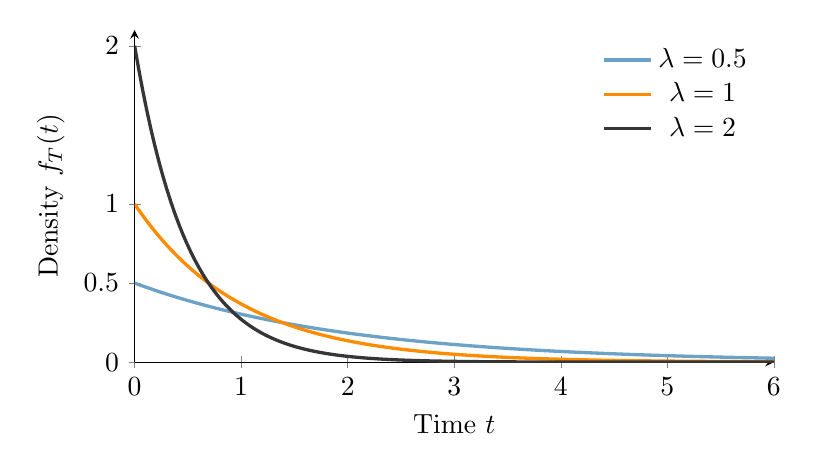
\begin{tikzpicture}
\begin{axis}[
    width=0.80\textwidth,
    height=5.8cm,
    xmin=0,xmax=6,
    ymin=0,ymax=2.1,
    axis lines=left,
    xlabel={Time $t$},
    ylabel={Density $f_T(t)$},
    ytick={0,0.5,1,2},
    legend style={draw=none,fill=none,at={(0.98,0.98)},anchor=north east}
]
\addplot[very thick,staViaBlue,domain=0:6,samples=160] {0.5*exp(-0.5*x)};
\addlegendentry{$\lambda=0.5$}
\addplot[very thick,staOrange,domain=0:6,samples=160] {exp(-x)};
\addlegendentry{$\lambda=1$}
\addplot[very thick,staDarkText,domain=0:6,samples=160] {2*exp(-2*x)};
\addlegendentry{$\lambda=2$}
\end{axis}
\end{tikzpicture}
\caption{Exponential densities for three rates. Increasing $\lambda$ concentrates more probability near zero and decreases the mean waiting time.}
\label{fig:exponential-densities}
\end{figure}

\begin{theorem}{Mean, Variance, and Quantiles of an Exponential Variable}
If $T\sim\operatorname{Exp}(\lambda)$, then
\[
    E[T]=\frac{1}{\lambda},
    \qquad
    \operatorname{Var}(T)=\frac{1}{\lambda^2}.
\]
Its $p$-quantile is
\[
    q_p=-\frac{\ln(1-p)}{\lambda},
    \qquad 0<p<1.
\]
\end{theorem}

The mean and standard deviation are both $1/\lambda$. The distribution is therefore strongly right-skewed: most waiting times are relatively short, but occasional long waits remain possible.

\begin{example}[ Time until the Next Server Request]\par
A server receives requests at a stable rate of 25 requests per second. Suppose the time $T$ until the next request is modelled as
\[
    T\sim\operatorname{Exp}(25),
\]
with time measured in seconds. The mean waiting time is
\[
    E[T]=\frac{1}{25}=0.04\text{ s}=40\text{ ms}.
\]
The probability of waiting more than 10 ms is
\[
\begin{aligned}
P(T>0.01)
  &=e^{-25(0.01)}\\
  &=e^{-0.25}\\
  &\approx0.7788.
\end{aligned}
\]
The 95th percentile is
\[
\begin{aligned}
q_{0.95}
  &=-\frac{\ln(0.05)}{25}\\
  &\approx0.1198\text{ s}\\
  &=119.8\text{ ms}.
\end{aligned}
\]
Thus 95\% of interarrival times are no more than approximately 119.8 ms under the constant-rate model.
\end{example}

\subsection{Memorylessness}

The exponential distribution has a distinctive property: after a waiting time has already elapsed, the distribution of the additional waiting time is unchanged.

\begin{theorem}{Memoryless Property}
If $T\sim\operatorname{Exp}(\lambda)$, then for $s,t\geq0$,
\[
    P(T>s+t\mid T>s)=P(T>t).
\]
The exponential distribution is said to be \textbf{memoryless}.
\end{theorem}

Memorylessness does not say that the same physical component becomes new again. It states that the model assigns the same distribution to its remaining life after survival to age $s$. This is appropriate only when the event rate does not change with age.

\begin{example}[ Remaining Component Life]\par
Suppose the operating life $T$ of an electronic component is exponentially distributed with mean 500 hours. The rate is
\[
    \lambda=\frac{1}{500}=0.002\text{ per hour}.
\]
The unconditional probability of surviving beyond 600 hours is
\[
    P(T>600)=e^{-0.002(600)}=e^{-1.2}\approx0.3010.
\]
Now suppose the component has already survived 400 hours. The probability that its total life exceeds 600 hours is the probability of surviving an additional 200 hours:
\[
\begin{aligned}
P(T>600\mid T>400)
  &=P(T>200)\\
  &=e^{-0.002(200)}\\
  &=e^{-0.4}\\
  &\approx0.6703.
\end{aligned}
\]
The conditional probability is larger than the unconditional probability because the component is known to have survived the first 400 hours. Under the exponential model, however, those 400 hours do not change the distribution of its additional lifetime.
\end{example}

\subsection{The connection with Poisson counts}

The Poisson and exponential distributions describe two views of the same constant-rate mechanism. A Poisson variable counts events in a fixed interval; an exponential variable measures the waiting time until the next event.

Suppose events occur independently at a constant rate $\lambda$ per unit time. If $N(t)$ denotes the number of events in an interval of length $t$, then
\[
    N(t)\sim\operatorname{Pois}(\lambda t).
\]
The waiting time $T$ until the first event exceeds $t$ exactly when no event occurs during the interval. Therefore,
\[
\begin{aligned}
P(T>t)
  &=P(N(t)=0)\\
  &=e^{-\lambda t},
\end{aligned}
\]
which is the exponential survival function.

\begin{example}[ Counts and Waiting Times for Network Traffic]\par
Return to a request rate of 25 per second and consider a 10 ms interval. The expected number of requests in the interval is
\[
    \lambda t=25(0.01)=0.25.
\]
Using the Poisson count model,
\[
    P(N(0.01)=0)=e^{-0.25}\approx0.7788.
\]
Using the exponential waiting-time model,
\[
    P(T>0.01)=e^{-25(0.01)}=e^{-0.25}\approx0.7788.
\]
The two calculations agree because ``no request in the next 10 ms'' and ``the next request arrives after more than 10 ms'' are the same event.
\end{example}

\subsection{Limitations of the exponential model}

An exponential lifetime model assumes a constant failure rate. It can describe sudden failures caused by independent random shocks, but it does not describe gradual wear, early manufacturing defects, or changing operating conditions unless those effects are negligible over the period studied.

Mechanical components often experience a changing failure rate: early failures may be caused by defects, a relatively stable middle period may follow, and wear may increase the failure rate later. A single exponential distribution cannot represent all three phases. The memoryless property is therefore both the model's defining feature and its strongest practical limitation.

\section{Choosing and Assessing a Continuous Model}
\label{sec:model-assessment-continuous}

A probability distribution is not selected only because its formula is familiar. Model choice begins with the measurement scale and the mechanism that could generate the observations. Graphical evidence then helps assess whether the proposed shape is credible.

\subsection{Comparing the three models}

\begin{table}[htbp]
\centering
\caption{Interpretive comparison of the three continuous models in this chapter.}
\label{tab:continuous-model-comparison}
\begin{tabularx}{\textwidth}{@{}l>{\raggedright\arraybackslash}X>{\raggedright\arraybackslash}X>{\raggedright\arraybackslash}X@{}}
\toprule
Model & Support and shape & Typical mechanism & Important limitation \\
\midrule
Uniform $U(a,b)$
& Bounded; constant density
& Equal-length intervals are equally likely
& Known bounds alone do not justify equal density \\
Normal $N(\mu,\sigma^2)$
& Entire real line; symmetric and bell-shaped
& Stable centre with many small sources of variation
& Can assign probability to impossible values and misses skewness or heavy tails \\
Exponential $\operatorname{Exp}(\lambda)$
& Nonnegative; right-skewed and decreasing
& Waiting time under a constant event rate
& Requires memorylessness and a constant rate \\
\bottomrule
\end{tabularx}
\end{table}

The supports provide an immediate first check. A uniform model needs meaningful lower and upper limits. A normal model permits negative and positive values. An exponential model permits only nonnegative values and begins with its highest density at zero. The shape and mechanism must then be considered together.

\begin{example}[ Selecting a Model from the Engineering Mechanism]\par
Consider the following quantities:
\begin{enumerate}
    \item a random activation time selected anywhere within a 20-minute testing window;
    \item the dimensional error from a centred and stable machining process;
    \item the time until the next alarm under a constant alarm rate.
\end{enumerate}
A uniform model is plausible for the deliberately randomised activation time because equal-length parts of the window are equally likely. A normal model may be plausible for the machining error because small independent sources of variation combine around a target. An exponential model may be plausible for the waiting time because the question concerns time to an event under a constant rate.

These choices are conditional, not automatic. Preferential scheduling would challenge the uniform model, tool wear could shift or skew the machining distribution, and a varying alarm rate would invalidate the exponential model.
\end{example}

\subsection{Graphical assessment}

A histogram can reveal support, skewness, multiple clusters, and extreme observations. A fitted density can be compared with the histogram, but agreement depends on the selected bin widths and may hide tail discrepancies. The empirical CDF gives another comparison because it shows accumulated proportions without bins.

No plot proves that a population follows a distribution. A sample contains limited information, and several models can look similar over the observed range. Graphs are diagnostics: they can expose important disagreements and indicate whether a model is a useful approximation for the intended decision.

\subsection{Quantile--quantile plots}

A quantile--quantile plot compares the ordered observations with quantiles expected under a proposed distribution. It is commonly abbreviated as a \textbf{QQ-plot}.

\begin{definition}{Quantile--Quantile Plot}
Let
\[
    x_{(1)}\leq x_{(2)}\leq\cdots\leq x_{(n)}
\]
be the ordered observations. For a proposed CDF $F$, define theoretical quantiles
\[
    q_i=F^{-1}\!\left(\frac{i-0.5}{n}\right),
    \qquad i=1,\ldots,n.
\]
A \textbf{QQ-plot} displays the pairs
\[
    (q_i,x_{(i)}).
\]
If the data follow the proposed location--scale family reasonably well, the points should lie approximately on a straight line.
\end{definition}

The plotting probabilities $(i-0.5)/n$ avoid using 0 and 1, whose quantiles may be infinite. Other closely related plotting conventions exist and lead to nearly the same diagnostic for moderate or large samples.

In a normal QQ-plot, an intercept reflects location and a slope reflects scale. Systematic curvature matters more than small random deviations. A few common patterns are:

\begin{itemize}
    \item approximately linear points: the normal shape may be a reasonable approximation;
    \item an upper end bending strongly above the line: the data have a longer right tail than the fitted normal model;
    \item both ends departing outward: the data may have heavier tails than the normal model;
    \item separated groups or abrupt changes in slope: the data may combine different populations.
\end{itemize}

\begin{figure}[htbp]
\centering
\begin{minipage}{0.48\textwidth}
\centering
\begin{tikzpicture}
\begin{axis}[
    width=\textwidth,
    height=5.5cm,
    xmin=-1.8,xmax=1.8,
    ymin=-1.8,ymax=1.8,
    axis lines=left,
    xlabel={Theoretical normal quantile},
    ylabel={Observed quantile},
    title={Approximately normal},
    xtick={-1,0,1},
    ytick={-1,0,1}
]
\addplot[dashed,staDarkText!60,domain=-1.6:1.6] {x};
\addplot[only marks,mark=*,mark size=2.1pt,staViaBlue] coordinates {
(-1.5,-1.43) (-1,-1.05) (-0.5,-0.46) (0,0.03) (0.5,0.48) (1,1.04) (1.5,1.46)};
\end{axis}
\end{tikzpicture}
\end{minipage}\hfill
\begin{minipage}{0.48\textwidth}
\centering
\begin{tikzpicture}
\begin{axis}[
    width=\textwidth,
    height=5.5cm,
    xmin=-1.8,xmax=1.8,
    ymin=-1.4,ymax=2.8,
    axis lines=left,
    xlabel={Theoretical normal quantile},
    ylabel={Observed quantile},
    title={Long right tail},
    xtick={-1,0,1},
    ytick={-1,0,1,2}
]
\addplot[dashed,staDarkText!60,domain=-1.6:1.6] {x};
\addplot[only marks,mark=*,mark size=2.1pt,staOrange] coordinates {
(-1.5,-0.92) (-1,-0.72) (-0.5,-0.42) (0,-0.08) (0.5,0.38) (1,1.22) (1.5,2.48)};
\end{axis}
\end{tikzpicture}
\end{minipage}
\caption{Schematic normal QQ-plots. Random scatter around a line is expected, whereas systematic curvature indicates a shape discrepancy.}
\label{fig:qq-patterns}
\end{figure}
\FloatBarrier

\begin{example}[ A Normal QQ-Plot for Response Times]\par
Seven ordered response times, in milliseconds, are
\[
    85,\ 91,\ 94,\ 98,\ 103,\ 111,\ 139.
\]
For $n=7$, the plotting probabilities are approximately
\[
    0.071,\ 0.214,\ 0.357,\ 0.500,\ 0.643,\ 0.786,\ 0.929.
\]
The corresponding standard normal quantiles are approximately
\[
    -1.47,\ -0.79,\ -0.37,\ 0,\ 0.37,\ 0.79,\ 1.47.
\]
Plotting the ordered response times against these theoretical quantiles would place the largest response, 139 ms, noticeably above the trend formed by the central observations. This suggests a longer right tail than a normal model would predict.

With only seven observations the evidence is weak, so the plot does not establish a different distribution. It does identify the upper tail as the part of the normal approximation that deserves further investigation, especially if high response-time percentiles are important.
\end{example}

\subsection{The purpose of a model}

Model adequacy depends on the question. A normal approximation that describes the centre well may still be unsuitable for estimating a very rare failure probability. An exponential model may describe short-term waiting times adequately while failing over a component's complete lifetime. The relevant range and consequence of model error should therefore guide how demanding the assessment must be.

A useful model combines three forms of evidence:
\begin{enumerate}
    \item the support agrees with possible values;
    \item the generating mechanism makes the distribution plausible;
    \item the observed data do not show a practically important disagreement with the proposed shape.
\end{enumerate}

Together, these models connect engineering thresholds with probabilities for practical decisions.


\part{Sampling and Statistical Inference}
\chapter{Sampling Distributions and the Central Limit Theorem}
\label{ch:sampling-distributions}

\section{Statistics as random variables}

\section{The sampling distribution of the mean}

\section{Standard error}

\section{The central limit theorem}

\chapter{Estimation and Confidence Intervals}
\label{ch:confidence-intervals}

\section{Estimators, estimates, bias, and precision}

\section{Intervals for a mean}

\section{Intervals for a proportion}

\section{Coverage and interpretation}

\chapter{Hypothesis Testing I: Principles and One-Sample Tests}
\label{ch:one-sample-tests}

\section{Engineering question and learning outcomes}
Does a process provide evidence against a specified target or baseline?

\section{Hypotheses, significance levels, and p-values}

\section{Type I and type II errors}

\section{One-sample tests for a mean and proportion}

\section{Effect size and practical importance}

\section{Python in practice}

\section{Common pitfalls and chapter summary}

\section{Exercises}

\chapter{Hypothesis Testing II: Comparing Two Groups}
\label{ch:two-group-tests}

\section{Independent and paired designs}

\section{Welch's two-sample t-test}

\section{The paired t-test}

\section{Comparing two proportions}

\chapter{Analysis of Variance}
\label{ch:anova}

Comparisons are not always limited to two groups. A production engineer may compare material from several suppliers, a software engineer may evaluate more than two caching strategies, and a climate engineer may compare energy use under several control settings. The response is quantitative in each case, but the explanatory variable identifies one of several groups.

It is tempting to compare every pair with a separate two-sample test. That approach creates two problems. First, the number of comparisons grows quickly: $k$ groups produce $k(k-1)/2$ pairs. Second, repeatedly testing at the same significance level increases the probability of making at least one type I error across the collection of comparisons. A procedure is needed that begins with one global question and, when appropriate, follows it with multiplicity-controlled comparisons.

\textbf{Analysis of variance}, abbreviated ANOVA, addresses the global question by comparing two sources of variation. Differences among group means create between-group variation, while natural differences among observations in the same group create within-group variation. If the between-group variation is large relative to the within-group variation, a model with one common population mean becomes difficult to reconcile with the data.

This chapter develops one-way ANOVA for independent groups. It explains the model, the decomposition of variation, the ANOVA table, the $F$ test, practical assumptions, and Tukey's method for identifying pairwise differences. Statistical software performs the arithmetic in realistic analyses, but the formulas reveal what the reported quantities mean and what conclusions they can support.

\section{From Two Groups to Several Groups}
\label{sec:anova-several-groups}

A one-way analysis has one quantitative response and one categorical explanatory variable. The categorical variable determines the groups being compared.

\begin{definition}{Factor and Levels}
A \textbf{factor} is a categorical explanatory variable used to divide observations into groups. Its possible categories are called the \textbf{levels} of the factor.
\end{definition}

In a supplier comparison, the factor may be supplier and its levels may be A, B, and C. In a software experiment, the factor may be caching strategy with levels no cache, local cache, and distributed cache. The word \emph{one-way} means that the analysis contains one factor. It does not mean that the hypothesis test is one-sided.

Let the factor have $k$ levels. Write $\mu_i$ for the population mean response at level $i$. One-way ANOVA tests
\[
H_0:\mu_1=\mu_2=\cdots=\mu_k
\]
against
\[
H_1:\text{not all of the population means are equal}.
\]
The alternative does not state that every mean differs from every other mean. It includes any configuration in which at least one pair of population means differs.

\begin{definition}{Omnibus Test}
An \textbf{omnibus test} assesses a global hypothesis involving several parameters. The one-way ANOVA $F$ test asks whether all group means can be represented by one common population mean; it does not by itself identify which means differ.
\end{definition}

This distinction determines the analysis order. The $F$ test addresses the global question. If the evidence indicates that the means are not all equal and the engineering question requires identification of particular groups, a post-hoc procedure addresses the pairwise questions while controlling error across the collection.

\subsection{Why separate pairwise tests are a poor default}

With three groups there are three pairwise comparisons. With five groups there are ten, and with ten groups there are 45. If every comparison is conducted as an unadjusted level-$\alpha$ test, the probability of at least one false rejection across the family is generally larger than $\alpha$. The exact probability depends on the dependence among the tests, so it is not correctly obtained by treating all pairwise statistics as independent.

ANOVA does not solve every multiple-comparison problem automatically. It provides one protected global test of equality. A compatible post-hoc procedure, such as Tukey's method, is still needed when the goal is to determine which pairs differ.

\section{The One-Way ANOVA Model}
\label{sec:one-way-anova-model}

Suppose level $i$ contributes $n_i$ observations,
\[
X_{i1},X_{i2},\ldots,X_{in_i},
\qquad i=1,\ldots,k.
\]
The total number of observations is
\[
N=\sum_{i=1}^{k}n_i.
\]
The group-means formulation of the one-way model is
\[
X_{ij}=\mu_i+\varepsilon_{ij},
\]
where $\mu_i$ is the population mean for level $i$ and $\varepsilon_{ij}$ is the random deviation of observation $j$ from that mean.

For the classical one-way ANOVA $F$ test, the errors are modelled as independent normal random variables with a common variance:
\[
\varepsilon_{ij}\sim N(0,\sigma^2).
\]
Equivalently,
\[
X_{ij}\sim N(\mu_i,\sigma^2).
\]
The means may differ across groups, but the classical model uses the same population variance in every group.

The sample mean for group $i$ is
\[
\bar x_i=\frac{1}{n_i}\sum_{j=1}^{n_i}x_{ij},
\]
and the grand mean of all $N$ observations is
\[
\bar x_{\cdot\cdot}
=\frac{1}{N}\sum_{i=1}^{k}\sum_{j=1}^{n_i}x_{ij}
=\frac{1}{N}\sum_{i=1}^{k}n_i\bar x_i.
\]
The second expression shows that the grand mean is a weighted average of the group means. Larger groups receive greater weight.

An observed within-group deviation is called a residual:
\[
e_{ij}=x_{ij}-\bar x_i.
\]
Residuals estimate the unobserved errors $\varepsilon_{ij}$. They are central to assessing whether the common-variance and normal-error descriptions are reasonable.

\begin{definition}{Balanced and Unbalanced Designs}
A one-way design is \textbf{balanced} when all group sample sizes are equal. It is \textbf{unbalanced} when at least two group sample sizes differ.
\end{definition}

Balance is not required, but it makes the group means contribute more symmetrically and often improves robustness when assumptions are only approximate. Unequal group sizes combined with unequal variances require particular care.

\subsection{The design comes before the model}

The observations must represent independent experimental or sampling units. Repeated measurements from the same machine, building, person, account, or component are not made independent by placing them in different groups in a data table. Clustered data and repeated-measures designs require methods beyond the one-way independent-groups model.

Random assignment of units to factor levels can support a causal interpretation when the experimental protocol is credible. In an observational comparison, ANOVA can describe evidence of an association between group membership and the mean response, but pre-existing group differences may provide alternative explanations. Random sampling and representative measurement determine how far the result can be generalised.

\begin{figure}[htbp]
\centering
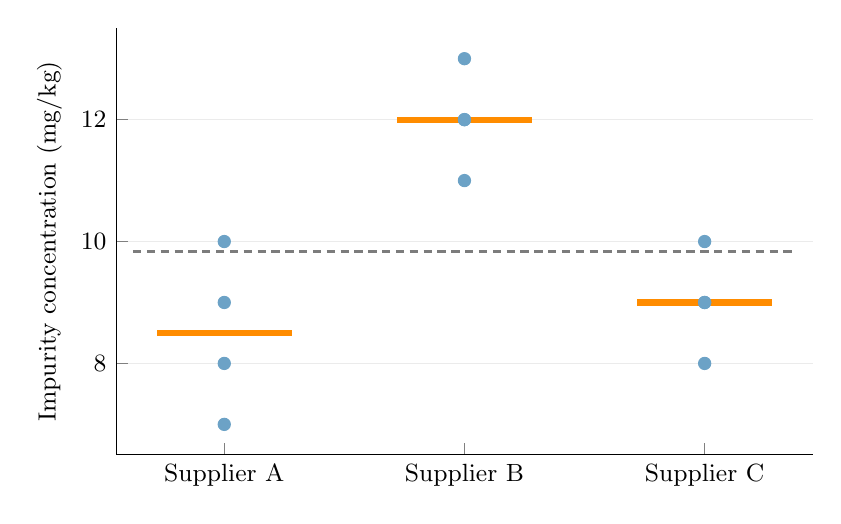
\begin{tikzpicture}
\begin{axis}[
  width=0.86\textwidth,
  height=7.0cm,
  xmin=0.55,xmax=3.45,
  ymin=6.5,ymax=13.5,
  xtick={1,2,3},
  xticklabels={Supplier A,Supplier B,Supplier C},
  ylabel={Impurity concentration (mg/kg)},
  axis x line*=bottom,
  axis y line*=left,
  ymajorgrids=true,
  grid style={staDarkText!10},
  tick label style={font=\small},
  label style={font=\small}
]
  \addplot[only marks,mark=*,mark size=2.2pt,staViaBlue]
    coordinates {(1,8) (1,9) (1,7) (1,10)};
  \addplot[only marks,mark=*,mark size=2.2pt,staViaBlue]
    coordinates {(2,12) (2,11) (2,13) (2,12)};
  \addplot[only marks,mark=*,mark size=2.2pt,staViaBlue]
    coordinates {(3,9) (3,10) (3,8) (3,9)};

  \draw[staOrange,line width=2.2pt] (axis cs:0.72,8.5) -- (axis cs:1.28,8.5);
  \draw[staOrange,line width=2.2pt] (axis cs:1.72,12.0) -- (axis cs:2.28,12.0);
  \draw[staOrange,line width=2.2pt] (axis cs:2.72,9.0) -- (axis cs:3.28,9.0);
  \draw[staDarkText!65,densely dashed,line width=1.0pt]
    (axis cs:0.62,9.833) -- (axis cs:3.38,9.833);
\end{axis}
\end{tikzpicture}
\caption{Observations from three groups. Blue points are individual measurements, orange segments are group means, and the dashed line is the grand mean. ANOVA compares the separation of the group means with the variation of observations around their own group means.}
\label{fig:anova-between-within}
\end{figure}

\FloatBarrier

\newpage

\section{Partitioning Variation and the \texorpdfstring{$F$}{F} Test}
\label{sec:anova-partition-f-test}

Every observation differs from the grand mean by an amount
\[
x_{ij}-\bar x_{\cdot\cdot}.
\]
This total deviation can be written as
\[
x_{ij}-\bar x_{\cdot\cdot}
=
(\bar x_i-\bar x_{\cdot\cdot})
+
(x_{ij}-\bar x_i).
\]
The first term is the deviation of the group mean from the grand mean. The second is the deviation of the observation from its own group mean. ANOVA turns this observation-level decomposition into a decomposition of squared variation.

\begin{definition}{ANOVA Sums of Squares}
The \textbf{total sum of squares} is
\[
SS_{\text{total}}
=\sum_{i=1}^{k}\sum_{j=1}^{n_i}
(x_{ij}-\bar x_{\cdot\cdot})^2.
\]
The \textbf{between-group sum of squares} is
\[
SS_{\text{between}}
=\sum_{i=1}^{k}n_i
(\bar x_i-\bar x_{\cdot\cdot})^2,
\]
and the \textbf{within-group sum of squares} is
\[
SS_{\text{within}}
=\sum_{i=1}^{k}\sum_{j=1}^{n_i}
(x_{ij}-\bar x_i)^2.
\]
\end{definition}

The group sizes appear in $SS_{\text{between}}$ because moving a group mean away from the grand mean affects every observation represented by that group. The within-group sum of squares is the sum of the squared residuals.

\begin{theorem}{ANOVA Sum-of-Squares Identity}
For any one-way dataset,
\[
SS_{\text{total}}
=SS_{\text{between}}+SS_{\text{within}}.
\]
The associated degrees of freedom satisfy
\[
N-1=(k-1)+(N-k).
\]
\end{theorem}

The identity is numerical and always holds for the stated definitions; it does not depend on normality. The distributional assumptions enter when the decomposition is used for inference.

Sums of squares grow with the number of independent pieces of information. Dividing by their degrees of freedom produces mean squares:
\[
MS_{\text{between}}
=\frac{SS_{\text{between}}}{k-1},
\qquad
MS_{\text{within}}
=\frac{SS_{\text{within}}}{N-k}.
\]
The within-group mean square is also called the error mean square. Under the classical model, it estimates the common variance $\sigma^2$ whether or not the group means are equal. When $H_0$ is true, the between-group mean square also estimates $\sigma^2$. If population means differ, $MS_{\text{between}}$ tends to be enlarged by their separation.

The resulting test statistic is
\[
F_{\mathrm{obs}}
=\frac{MS_{\text{between}}}{MS_{\text{within}}}.
\]
Values close to 1 indicate that the two variance estimates are of similar size. Large values indicate that the group means are more separated than would be expected from the observed within-group variation under one common population mean.

\subsection{The $F$ distribution}

An $F$ distribution is a continuous probability distribution for a ratio of two independent variance estimates after appropriate scaling. It takes only nonnegative values, is generally right-skewed, and is indexed by a numerator and a denominator number of degrees of freedom.

\begin{theorem}{One-Way ANOVA $F$ Test}
Under the classical one-way normal model and
\[
H_0:\mu_1=\mu_2=\cdots=\mu_k,
\]
the statistic
\[
F_{\mathrm{obs}}
=\frac{MS_{\text{between}}}{MS_{\text{within}}}
\]
is a realised value from an $F$ distribution with $k-1$ numerator and $N-k$ denominator degrees of freedom. The upper-tail $p$-value is
\[
p
=P\!\left(
F_{k-1,N-k}\geq F_{\mathrm{obs}}
\mid H_0\text{ and the model assumptions}
\right).
\]
\end{theorem}

Only the upper tail is relevant because evidence against equal means appears when the between-group mean square is unusually large relative to the within-group mean square. Statistical software evaluates the $F$ probability; an $F$ table is not required for routine analysis.

When there are exactly two groups and the equal-variance model is used, the one-way ANOVA statistic equals the square of the classical pooled two-sample $t$ statistic:
\[
F=t^2.
\]
Thus one-way ANOVA extends the equal-variance comparison of two means. It is not equivalent to Welch's unequal-variance two-sample procedure.

\subsection{The ANOVA table}

The calculations are conventionally organised as shown in \autoref{tab:anova-table-general}.

\begin{table}[htbp]
\centering
\caption{The classical one-way ANOVA table.}
\label{tab:anova-table-general}
\begin{tabular}{@{}lcccc@{}}
\toprule
Source & Sum of squares & df & Mean square & Statistic \\
\midrule
Between groups
& $SS_{\text{between}}$
& $k-1$
& $SS_{\text{between}}/(k-1)$
& $F=MS_{\text{between}}/MS_{\text{within}}$ \\
Within groups
& $SS_{\text{within}}$
& $N-k$
& $SS_{\text{within}}/(N-k)$
& \\
Total
& $SS_{\text{total}}$
& $N-1$
&
& \\
\bottomrule
\end{tabular}
\end{table}

The table is more than a software format. It records how the observed variation is partitioned and makes the construction of the test statistic visible.

\newpage

\begin{example}[ Impurity Concentrations from Three Suppliers]\par
A production engineer measures impurity concentration in four independently selected batches from each of three resin suppliers. The measurements, in mg/kg, are
\[
\begin{array}{c|cccc|c}
\text{Supplier} & \multicolumn{4}{c|}{\text{observations}} & \bar x_i\\
\hline
A & 8 & 9 & 7 & 10 & 8.5\\
B & 12 & 11 & 13 & 12 & 12.0\\
C & 9 & 10 & 8 & 9 & 9.0
\end{array}
\]
The grand mean is
\[
\bar x_{\cdot\cdot}
=\frac{8+9+7+10+12+11+13+12+9+10+8+9}{12}
=\frac{118}{12}
\approx9.833.
\]
The between-group sum of squares is
\[
\begin{aligned}
SS_{\text{between}}
&=4(8.5-9.833)^2
  +4(12.0-9.833)^2
  +4(9.0-9.833)^2\\
&\approx28.667.
\end{aligned}
\]
Within each supplier, the squared residuals sum to
\[
\begin{aligned}
SS_A&=(8-8.5)^2+(9-8.5)^2+(7-8.5)^2+(10-8.5)^2=5,\\
SS_B&=(12-12)^2+(11-12)^2+(13-12)^2+(12-12)^2=2,\\
SS_C&=(9-9)^2+(10-9)^2+(8-9)^2+(9-9)^2=2.
\end{aligned}
\]
Therefore,
\[
SS_{\text{within}}=5+2+2=9,
\]
and the sum-of-squares identity gives
\[
SS_{\text{total}}=28.667+9=37.667.
\]
With $k=3$ and $N=12$, the ANOVA table is
\[
\begin{array}{lrrrr}
\toprule
\text{Source} & SS & df & MS & F\\
\midrule
\text{Between groups} & 28.667 & 2 & 14.333 & 14.333\\
\text{Within groups}  &  9.000 & 9 &  1.000 & \\
\text{Total}          & 37.667 & 11 &       & \\
\bottomrule
\end{array}
\]
For
\[
H_0:\mu_A=\mu_B=\mu_C,
\]
the statistic $F=14.333$ has $2$ and $9$ degrees of freedom under $H_0$. The upper-tail probability is approximately
\[
p=0.0016.
\]
The data provide evidence that the three population mean impurity concentrations are not all equal. The result does not yet establish which suppliers differ, nor whether supplier membership caused the differences. Those conclusions require pairwise inference and consideration of the design.
\end{example}

\newpage

\section{Assumptions, Diagnostics, and Robustness}
\label{sec:anova-assumptions}

The exact classical $F$ result follows from independent normal errors with a common variance. Practical validity depends on how the data were generated as well as on the observed distributions. \autoref{tab:anova-conditions} translates the model into questions that can be investigated.

\begin{table}[htbp]
\centering
\caption{Conditions to examine before interpreting a one-way ANOVA.}
\label{tab:anova-conditions}
\begin{tabularx}{\textwidth}{@{}l>{\raggedright\arraybackslash}X@{}}
\toprule
Condition & Practical question \\
\midrule
Quantitative response & Is a population mean meaningful for the measured outcome in every group? \\
Independent observations & Are different rows genuinely independent experimental or sampling units rather than repeated, clustered, or time-dependent measurements? \\
Representative or randomised design & Do the observations support generalisation to the target populations, or were units randomly assigned so that a causal comparison is credible? \\
Approximately normal errors & Within each group, are residuals reasonably compatible with a normal model, especially when group sizes are small? \\
Common population variance & Are the within-group spreads sufficiently similar for one pooled variance to represent all groups? \\
Comparable measurement & Were definitions, instruments, timing, censoring, and missing-data handling comparable across levels? \\
\bottomrule
\end{tabularx}
\end{table}

\subsection{Independence and study design}

Independence cannot be diagnosed reliably from a histogram, boxplot, or normality test. It follows from the sampling and experimental structure. Treating repeated observations from one unit as independent creates artificial information and usually makes standard errors too small. No transformation of the response repairs an invalid independence assumption.

The observational unit must therefore be stated explicitly. If four measurements are taken from each of ten components, the study has ten independently sampled components unless the model accounts for the repeated measurements within component. It does not automatically have 40 independent components.

\subsection{Normality concerns the errors within groups}

The classical model describes the distribution around each group mean. Consequently, the relevant quantities are the residuals $e_{ij}=x_{ij}-\bar x_i$, not the overall response distribution formed by mixing all groups. Even perfectly normal groups can produce a multimodal combined distribution when their means differ.

Group plots and residual plots can reveal strong skewness, outliers, and unequal spread. A normal quantile plot of the residuals can provide an additional diagnostic. Formal normality tests are not a mechanical gatekeeper: they may have little power in small samples and detect immaterial deviations in large samples.

Classical ANOVA is often reasonably robust to moderate non-normality when group sizes are not very small and the design is balanced or nearly balanced. Severe skewness, influential outliers, heavy tails, dependence, or censoring can still undermine a mean-based analysis. There is no universal sample-size rule that overrides these features.

\subsection{Common variance and unequal group sizes}

The pooled within-group mean square assumes one population variance $\sigma^2$. Similar-looking sample standard deviations do not prove equality, and a preliminary variance test should not automatically decide which analysis is reported. The judgment should combine subject-matter knowledge, study design, group sizes, and plots of the group or residual distributions.

Unequal variances are most problematic when group sizes are also unequal. In particular, a small high-variance group or a large low-variance group can distort the classical $F$ test. A balanced design provides protection because each group contributes comparably, but balance does not make extreme variance differences irrelevant.

\begin{custombox}{When the group variances are not similar}
Welch's one-way ANOVA provides a practical alternative when independent groups have unequal variances. It weights the group information differently and uses adjusted degrees of freedom; statistical software performs the calculation. If pairwise follow-up is needed after Welch's ANOVA, Games--Howell comparisons provide the corresponding unequal-variance approach. Ordinary Tukey comparisons use the pooled within-group variance and should not be combined automatically with a Welch omnibus analysis.
\end{custombox}

Welch's ANOVA and Games--Howell are included here as method-selection tools, not as additional hand-calculation procedures. Transformations or rank-based methods may sometimes be suitable, but they change the modelling or interpretation and are outside the core scope of this chapter.

\section{Post-Hoc Comparisons and Effect Magnitude}
\label{sec:anova-posthoc-effect}

A significant omnibus result supports the statement that the population means are not all equal. It does not support statements such as ``supplier B differs from supplier A'' without a comparison designed for that pair. Inspecting the largest sample means after the test and then applying ordinary unadjusted $t$ intervals ignores the selection and multiplicity that produced the question.

\subsection{Family-wise error and Tukey's method}

The \textbf{family-wise error rate} is the probability of making at least one type I error among a specified family of comparisons. Tukey's method constructs simultaneous inference for every pair of population means while controlling this probability at a chosen level $\alpha$ under the classical one-way model.

\begin{theorem}{Tukey--Kramer Pairwise Confidence Intervals}
For all pairwise differences $\mu_i-\mu_j$ in a classical one-way ANOVA, a simultaneous $100(1-\alpha)\%$ Tukey--Kramer confidence interval is
\[
(\bar x_i-\bar x_j)
\pm
q_{1-\alpha;k,N-k}
\sqrt{
\frac{MS_{\text{within}}}{2}
\left(\frac{1}{n_i}+\frac{1}{n_j}\right)
},
\]
where $q_{1-\alpha;k,N-k}$ is a critical value from the studentized-range distribution. When all group sizes equal $n$, the margin of error reduces to
\[
q_{1-\alpha;k,N-k}
\sqrt{\frac{MS_{\text{within}}}{n}}.
\]
\end{theorem}

Statistical software evaluates the studentized-range critical value and usually reports multiplicity-adjusted $p$-values together with simultaneous confidence intervals. A pair is distinguished at family-wise level $\alpha$ when its simultaneous interval excludes zero.

The usual exploratory workflow begins with the omnibus question and, when group identification is relevant, follows it with Tukey comparisons. The protection in a Tukey family comes from its simultaneous critical value, not merely from performing an $F$ test first. Comparisons formulated in advance to answer specific engineering questions are a different design problem and lie outside this introductory treatment.

\begin{example}[ Locating the Supplier Differences]\par
Return to the impurity data from the preceding example. Since all three groups have size $n=4$ and $MS_{\text{within}}=1$, the 95\% Tukey margin of error is
\[
q_{0.95;3,9}\sqrt{\frac{1}{4}}
\approx3.948(0.5)
=1.974\text{ mg/kg}.
\]
The pairwise results are
\[
\begin{array}{lrrrl}
\toprule
\text{Difference} & \text{estimate} & \multicolumn{2}{c}{\text{95\% simultaneous interval}} & \text{adjusted }p\\
\midrule
\mu_B-\mu_A &  3.50 & [ &  1.526,\ 5.474] & 0.0020\\
\mu_C-\mu_A &  0.50 & [ & -1.474,\ 2.474] & 0.7655\\
\mu_C-\mu_B & -3.00 & [ & -4.974,-1.026] & 0.0055\\
\bottomrule
\end{array}
\]
At the 5\% family-wise level, supplier B differs from both A and C, while A and C are not distinguished. The intervals also quantify the differences: supplier B's mean impurity concentration is estimated to exceed A's by between about 1.5 and 5.5 mg/kg and C's by between about 1.0 and 5.0 mg/kg. Failure to distinguish A and C does not establish that their population means are identical.
\end{example}

\subsection{A descriptive effect size}

The omnibus $p$-value measures incompatibility with equal means under the model; it does not measure how important the group effect is. A simple descriptive effect size is
\[
\eta^2
=\frac{SS_{\text{between}}}{SS_{\text{total}}}.
\]
It is the proportion of the observed total sum of squares represented by differences among the observed group means. For the supplier example,
\[
\eta^2
=\frac{28.667}{37.667}
\approx0.761.
\]
Thus about 76.1\% of the observed squared variation in this small illustrative dataset is associated with supplier-level mean differences.

This value is a sample description, not the probability that supplier determines an individual measurement and not automatically the proportion causally explained by supplier. It can overstate the corresponding population effect, especially in small samples. Group means, pairwise differences, and their confidence intervals remain essential because they retain the engineering units of the response.

\newpage

\section{Choosing and Reporting a One-Way Analysis}
\label{sec:anova-reporting}

The method must match both the data structure and the engineering question. A classical one-way ANOVA is appropriate for a quantitative response from independent groups when a common within-group variance is a credible approximation. Welch's ANOVA is preferable when the independent groups have materially different variances. Neither method applies directly to paired, repeated, clustered, or time-dependent observations.

\begin{custombox}{Seven-step analysis order for several means}
A defensible one-way analysis proceeds in this order:
\begin{enumerate}
  \item state the target population, observational unit, quantitative response, factor, and factor levels;
  \item explain how units were sampled or assigned and whether the groups contain independent observations;
  \item report group sample sizes, means, standard deviations, and a plot showing distributions and possible outliers;
  \item assess whether the classical common-variance model is adequate or whether Welch's unequal-variance approach is more credible;
  \item report the omnibus hypotheses, test statistic with degrees of freedom, $p$-value, and an effect magnitude;
  \item when particular pairs must be identified, use a compatible multiplicity-controlled procedure and report simultaneous confidence intervals; and
  \item interpret differences in engineering units, including uncertainty, practical importance, design limitations, and the distinction between association and causation.
\end{enumerate}
\end{custombox}

For the illustrative supplier data, a compact report could read:

\begin{quote}
Mean impurity concentration differed among the three sampled suppliers, $F(2,9)=14.33$, $p=0.0016$, with $\eta^2=0.761$ in this sample. Tukey 95\% simultaneous intervals indicated that supplier B had a higher population mean than A by an estimated 3.50 mg/kg, 95\% simultaneous CI $[1.53,5.47]$, and a higher mean than C by an estimated 3.00 mg/kg, 95\% simultaneous CI $[1.03,4.97]$. Suppliers A and C were not distinguished. The result concerns the sampled production conditions; a causal supplier effect requires a design that rules out systematic differences in batches, handling, and measurement.
\end{quote}

The report combines the global question, the pairwise questions, effect magnitude, uncertainty, and design limitations. Reporting only ``ANOVA was significant'' omits the quantities needed for an engineering decision. Conversely, presenting many pairwise decisions without the family and adjustment obscures the error rate being controlled.

One-way ANOVA therefore has a clear division of labour. The variance decomposition explains the global $F$ test, multiplicity-controlled intervals locate relevant group differences, and study design determines what those numerical results can mean. The next chapter replaces categorical group membership with a quantitative explanatory variable and develops simple linear regression.


\part{Modelling and Integrated Analysis}
\chapter{Simple Linear Regression}
\label{ch:linear-regression}

\section{The regression model and least squares}

\section{Correlation and coefficient of determination}

\section{Inference for the slope}

\section{Residual diagnostics and prediction}

\chapter{Categorical Data and Chi-Square Tests}
\label{ch:categorical-data}

Engineering data are not always measurements on a numerical scale. A software incident may be classified by cause, a building component by condition, a production fault by type, and a shipment by destination and delivery status. Such categories are often summarised by counts and proportions rather than means and standard deviations.

Categorical analysis asks whether observed counts are compatible with a proposed probability model. A goodness-of-fit analysis compares one categorical distribution with specified probabilities. A contingency-table analysis compares two classifications and asks whether their distributions are associated. In both settings, Pearson's chi-square statistic measures discrepancies between observed and expected counts.

The arithmetic is compact, but a useful analysis requires more than a test statistic. The statistical question must match the sampling design, expected counts must support the chi-square approximation, and a significant result must be followed by an examination of where and how the counts differ. Effect magnitude and conditional proportions are essential because a small $p$-value does not by itself describe engineering importance.

This chapter develops goodness-of-fit tests with specified and estimated parameters, Monte Carlo assessment, tests of independence and homogeneity, residual interpretation, Cram\'er's $V$, sparse-table alternatives, and a practical reporting workflow. Statistical software normally performs the calculations; the objective here is to understand the quantities it reports and the conclusions they can support.

\section{Categorical Counts and Statistical Questions}
\label{sec:categorical-questions}

\begin{definition}{Categorical Variable and Frequency}
A \textbf{categorical variable} assigns each observational unit to one of a set of categories. The \textbf{frequency} of a category is the number of observed units assigned to it. Dividing a frequency by the total number of units gives a sample proportion.
\end{definition}

Categories may be nominal, such as defect mechanism or material type, or ordered, such as low, medium, and high severity. The methods in this chapter use the category counts. They do not treat category labels as numerical measurements, even when the labels happen to be coded as $0,1,2,\ldots$.

A valid count table begins with clearly defined observational units. Each unit should contribute to exactly one category in a one-way table and exactly one cell in a two-way table. Categories should be mutually exclusive, collectively adequate for the stated population, and defined before discrepancies in the data are examined. Repeated observations from the same machine, person, site, or time series may be dependent and cannot automatically be treated as separate independent units.

Three related questions must be distinguished.

\begin{table}[htbp]
\centering
\caption{Three categorical questions and their data structures.}
\label{tab:categorical-questions}
\begin{tabularx}{\textwidth}{@{}p{0.20\textwidth}>{\raggedright\arraybackslash}X>{\raggedright\arraybackslash}X@{}}
\toprule
Question & Data structure & Null hypothesis \\
\midrule
Goodness of fit & One sample classified into $k$ categories & The population category probabilities equal a specified distribution \\
Independence & One sample; two categorical variables recorded on every unit & The two population classifications are independent \\
Homogeneity & Independent samples from several populations or groups & The populations have the same categorical distribution \\
\bottomrule
\end{tabularx}
\end{table}

A test of independence and a test of homogeneity use the same Pearson calculation for a contingency table. Their interpretations differ because their data-generating designs differ. If one random sample of components is classified by both supplier and defect status, the question is independence. If separate samples are taken from several suppliers and their defect distributions are compared, the question is homogeneity.

Counts and proportions play complementary roles. Counts determine the sampling variation and enter the chi-square statistic. Proportions show the size and pattern of differences. Applying a chi-square test to a table containing percentages without the corresponding sample sizes loses the information needed to assess sampling variation.

\section{Chi-Square Goodness of Fit}
\label{sec:chi-square-goodness-fit}

Suppose a sample of $n$ independent units is classified into $k$ categories. Let $O_i$ be the observed count in category $i$. A fully specified null model gives category probabilities
\[
p_{1,0},p_{2,0},\ldots,p_{k,0},
\qquad
\sum_{i=1}^{k}p_{i,0}=1.
\]
The hypotheses are
\[
H_0:p_i=p_{i,0}\quad\text{for every }i
\]
against
\[
H_1:\text{at least one population category probability differs from its specified value}.
\]
Under $H_0$, the expected count in category $i$ is
\[
E_i=np_{i,0}.
\]

\begin{definition}{Pearson Chi-Square Statistic}
The \textbf{Pearson chi-square statistic} compares observed and expected counts:
\[
\chi^2_{\mathrm{obs}}
=\sum_{i=1}^{k}\frac{(O_i-E_i)^2}{E_i}.
\]
Every term is nonnegative. A category contributes strongly when its observed count is far from its expected count relative to the size of that expected count.
\end{definition}

Each summand is the square of a standardised count discrepancy,
\[
\frac{(O_i-E_i)^2}{E_i}
=
\left(\frac{O_i-E_i}{\sqrt{E_i}}\right)^2.
\]
Under $H_0$, category counts fluctuate around their expected counts. When the expected counts are sufficiently large, the vector of count discrepancies is approximately multivariate normal. The discrepancies are correlated and are constrained because
\[
\sum_{i=1}^{k}(O_i-E_i)=0.
\]
Consequently, only $k-1$ independent discrepancy directions remain. After accounting for the covariance among the counts, Pearson's quadratic form is asymptotically equivalent to a sum of squares of $k-1$ independent standard normal directions. \hyperref[sec:chi-square-sample-variance]{Section~\ref*{sec:chi-square-sample-variance}} introduced exactly such a sum of squared standard normal variables as a chi-square distribution. This explains the $k-1$ degrees of freedom in the following approximation without requiring the categorical observations themselves to be normally distributed.

The category observations themselves are not chi-square distributed. It is the sampling distribution of Pearson's discrepancy statistic, calculated under $H_0$, that is approximately chi-square. The statistic equals zero only when every observed count equals its expected count. Increasing discrepancies produce larger values, so goodness-of-fit tests use the upper tail of the reference distribution.

\Needspace{9\baselineskip}
\begin{theorem}{Goodness-of-Fit Chi-Square Approximation}
If the null probabilities are fully specified, the observations are independent, and the expected counts are sufficiently large, then under $H_0$,
\[
\chi^2_{\mathrm{obs}}
\quad\text{is approximately distributed as}\quad
\chi^2_{k-1}.
\]
The approximate $p$-value is
\[
P\!\left(\chi^2_{k-1}\geq\chi^2_{\mathrm{obs}}\mid H_0\right).
\]
\end{theorem}

The $k-1$ degrees of freedom reflect the fixed total count: after $k-1$ category counts are known, the final count is determined by their sum. A conservative introductory guideline is to require every expected count to be at least 5. This is a practical approximation guideline, not a mathematical law. It concerns expected counts, not observed counts.

\begin{example}[ Automated Inspection Profile]\par
Historical validation of an automated inspection system gives the following probabilities for four mutually exclusive defect classifications. A new production period contains 400 independently inspected defective components.

\begin{center}
\begin{tabular}{lrrrr}
\toprule
Category & Alignment & Contamination & Solder & Other \\
\midrule
Specified probability $p_{i,0}$ & 0.45 & 0.30 & 0.15 & 0.10 \\
Observed count $O_i$ & 212 & 96 & 58 & 34 \\
Expected count $E_i$ & 180 & 120 & 60 & 40 \\
$(O_i-E_i)^2/E_i$ & 5.689 & 4.800 & 0.067 & 0.900 \\
\bottomrule
\end{tabular}
\end{center}

All expected counts exceed 5. The test statistic is
\[
\chi^2_{\mathrm{obs}}
=5.689+4.800+0.067+0.900
=11.456.
\]
No parameters were estimated from the new data, so $df=4-1=3$. The upper-tail probability is
\[
p=P(\chi^2_3\geq11.456)\approx0.0095.
\]
At the 5\% level, the specified historical profile is rejected. The largest contributions come from alignment and contamination: alignment defects occur more often than expected and contamination defects less often. The test does not show why the profile changed, whether the inspection system or the production process changed, or whether every difference is operationally important.
\end{example}

\begin{figure}[htbp]
\centering
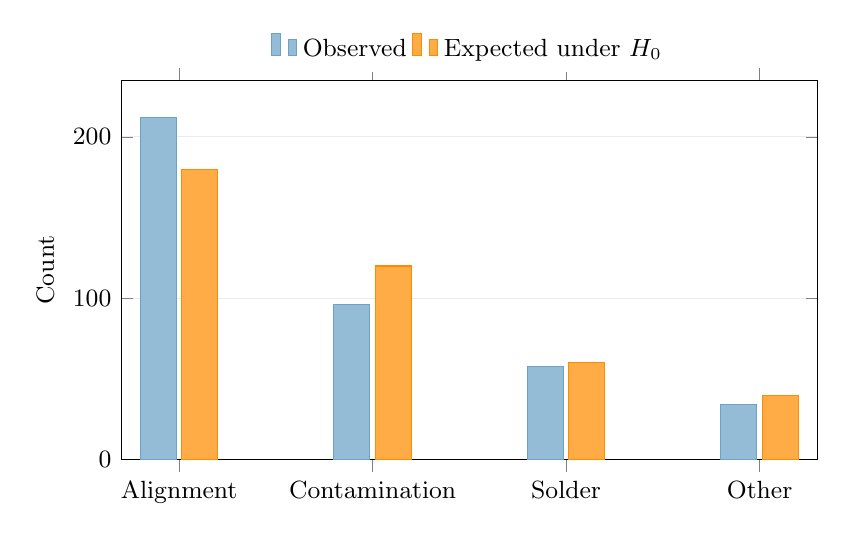
\begin{tikzpicture}
\begin{axis}[
  width=0.86\textwidth,
  height=6.4cm,
  ybar=2pt,
  bar width=13pt,
  ymin=0,
  ymax=235,
  ylabel={Count},
  symbolic x coords={Alignment,Contamination,Solder,Other},
  xtick=data,
  tick label style={font=\small},
  label style={font=\small},
  legend style={at={(0.5,1.02)},anchor=south,legend columns=2,draw=none,font=\small},
  ymajorgrids=true,
  grid style={staDarkText!10}
]
\addplot[fill=staViaBlue!72,draw=staViaBlue] coordinates {
  (Alignment,212) (Contamination,96) (Solder,58) (Other,34)
};
\addlegendentry{Observed}
\addplot[fill=staOrange!72,draw=staOrange] coordinates {
  (Alignment,180) (Contamination,120) (Solder,60) (Other,40)
};
\addlegendentry{Expected under $H_0$}
\end{axis}
\end{tikzpicture}
\caption{Observed and expected defect counts for the inspection-profile example. The chi-square statistic combines the category discrepancies after scaling them by their expected counts.}
\label{fig:gof-observed-expected}
\end{figure}

\FloatBarrier

\section{Estimated Parameters, Pooling, and Simulation}
\label{sec:chi-square-estimated-simulation}

A goodness-of-fit null hypothesis may specify a family of distributions without specifying all its parameters. For example, the claim may be that event counts follow a Poisson distribution with an unknown rate. Estimating that rate from the same sample makes the fitted expected counts closer to the observations and consumes information that would otherwise contribute to the goodness-of-fit assessment.

\begin{theorem}{Degrees of Freedom with Estimated Parameters}
Suppose a goodness-of-fit analysis uses $k$ final categories and estimates $m$ independent parameters from the same data under regular model conditions. The usual chi-square reference distribution has
\[
df=k-1-m.
\]
The parameter-estimation procedure and the expected-count calculation must correspond to the stated null model.
\end{theorem}

The subtraction of $m$ is not optional bookkeeping. Using $k-1$ after fitting parameters from the data generally gives the wrong reference distribution and therefore the wrong $p$-value.

\subsection{Pooling categories}

Distributional models often contain tail categories with small expected counts. Adjacent or scientifically compatible categories may be pooled so that the approximation is more credible. Observed counts and null probabilities must be pooled in exactly the same way, and the number $k$ refers to the final pooled categories.

Pooling should be based on the measurement scale and the expected counts, not on which observed discrepancies are inconvenient. The final category should include the entire remaining tail probability. Omitting rare outcomes makes the expected probabilities sum to less than one and changes the null model.

\begin{example}[ Poisson Model for Service Alerts]\par
A monitoring team records the number of service alerts in each of 200 independent 15-minute intervals. The ungrouped data give sample mean $\hat\lambda=3.49$ alerts per interval. To assess a Poisson model, counts of 7 or more are pooled into one tail category.

\begin{center}
\small
\begin{tabular}{lrrrrrrrr}
\toprule
Alerts & 0 & 1 & 2 & 3 & 4 & 5 & 6 & $7+$ \\
\midrule
Observed $O_i$ & 11 & 17 & 36 & 38 & 42 & 27 & 17 & 12 \\
Expected $E_i$ & 6.10 & 21.29 & 37.15 & 43.22 & 37.71 & 26.32 & 15.31 & 12.90 \\
\bottomrule
\end{tabular}
\end{center}

For $i=0,\ldots,6$, the expected counts are
\[
E_i=200\,P\!\left(X=i\right),
\qquad X\sim\operatorname{Pois}(3.49),
\]
and the final expected count is
\[
E_{7+}=200\,P(X\geq7).
\]
The minimum expected count is 6.10. With $k=8$ final categories and $m=1$ estimated parameter,
\[
df=8-1-1=6.
\]
The test gives
\[
\chi^2_{\mathrm{obs}}=6.222,
\qquad
p=P(\chi^2_6\geq6.222)\approx0.399.
\]
The data do not provide evidence against the fitted Poisson model. This conclusion does not prove that alert counts are Poisson. Dependence across adjacent intervals, changing traffic levels, or unmodelled incident periods may still make the model unsuitable for operational use.
\end{example}

\subsection{Monte Carlo assessment under the null model}

When the chi-square approximation is doubtful, or when its adequacy is itself of interest, the null distribution of the statistic can be approximated by simulation. This preserves the same hypothesis-testing logic while replacing the theoretical reference curve with statistics generated under the null model.

\begin{custombox}{Monte Carlo goodness-of-fit assessment}
For an observed statistic $T_{\mathrm{obs}}$ and $B$ simulated samples:
\begin{enumerate}
  \item specify or fit the null distribution exactly as in the observed analysis;
  \item simulate $B$ samples of the same size under that null model;
  \item if parameters were estimated from the observed data, repeat the parameter estimation and expected-count construction within every simulated sample;
  \item calculate a statistic $T_b$ for each simulated sample; and
  \item estimate the upper-tail probability by
  \[
  \hat p_{\mathrm{MC}}
  =\frac{1+\#\{b:T_b\geq T_{\mathrm{obs}}\}}{B+1}.
  \]
\end{enumerate}
\end{custombox}

The added 1 prevents an estimated $p$-value of exactly zero and recognises that the observed dataset is one possible outcome under the null comparison. For the fully specified inspection profile in \hyperref[fig:gof-observed-expected]{Figure~\ref*{fig:gof-observed-expected}}, 200,000 multinomial simulations give an estimated upper-tail probability of about 0.0095, close to the chi-square approximation.

Simulation addresses the reference distribution, not defects in the study. It cannot repair dependent observations, categories chosen after inspecting the discrepancies, measurement errors, or a null model that fails to represent the scientific question.

\section{Contingency Tables: Independence and Homogeneity}
\label{sec:chi-square-contingency}

A two-way table cross-classifies observations using a row variable and a column variable. Let $O_{ij}$ be the observed count in row $i$ and column $j$, with $r$ rows, $c$ columns, and total sample size $n$.

\begin{definition}{Contingency Table and Margins}
A \textbf{contingency table} displays counts for combinations of two categorical variables. Row totals and column totals are called the \textbf{margins}. Conditional proportions divide cell counts by the relevant row or column total and describe the categorical distribution within a group.
\end{definition}

For an independence analysis, write $p_{ij}$ for the population probability of cell $(i,j)$, $p_{i+}$ for the row probability, and $p_{+j}$ for the column probability. The hypotheses are
\[
H_0:p_{ij}=p_{i+}p_{+j}\quad\text{for every cell}
\]
against
\[
H_1:\text{the two population classifications are associated}.
\]
Under independence, the expected cell count is estimated from the margins:
\[
E_{ij}
=\frac{(\text{row }i\text{ total})(\text{column }j\text{ total})}{n}.
\]

For a homogeneity analysis, the null hypothesis states that all sampled populations have the same column-category probabilities. The expected-count formula and Pearson statistic are the same; only the sampling design and contextual wording differ.

\begin{theorem}{Pearson Test for a Contingency Table}
For an $r\times c$ table with independent observational units and sufficiently large expected counts,
\[
\chi^2_{\mathrm{obs}}
=\sum_{i=1}^{r}\sum_{j=1}^{c}
\frac{(O_{ij}-E_{ij})^2}{E_{ij}}
\]
has, under the null hypothesis, an approximate chi-square distribution with
\[
df=(r-1)(c-1).
\]
\end{theorem}

The degrees of freedom account for the estimated row and column margins. The same conservative expected-count guideline can be used: every expected cell count should preferably be at least 5 for the introductory Pearson approximation.

\begin{example}[ Defect Profiles Across Production Lines]\par
A plant independently samples 120 defect records from each of three production lines. Each defect is classified as alignment, contamination, solder, or other.

\Needspace{9\baselineskip}
\begin{center}
\textbf{Observed defect counts}\par\medskip
\begin{tabular}{lrrrrr}
\toprule
Line & Alignment & Contamination & Solder & Other & Total \\
\midrule
L1 & 25 & 40 & 15 & 40 & 120 \\
L2 & 40 & 25 & 15 & 40 & 120 \\
L3 & 55 & 10 & 10 & 45 & 120 \\
\midrule
Total & 120 & 75 & 40 & 125 & 360 \\
\bottomrule
\end{tabular}
\end{center}

Because separate samples were taken from the three lines, the design asks whether the defect-type distributions are homogeneous. The null hypothesis states that all three lines have the same four category probabilities. For example,
\[
E_{\mathrm{L1,Alignment}}
=\frac{120(120)}{360}
=40.
\]
The expected table is
\[
\begin{array}{lrrrr}
\toprule
 & \text{Alignment} & \text{Contamination} & \text{Solder} & \text{Other}\\
\midrule
\text{L1} & 40.00 & 25.00 & 13.33 & 41.67\\
\text{L2} & 40.00 & 25.00 & 13.33 & 41.67\\
\text{L3} & 40.00 & 25.00 & 13.33 & 41.67\\
\bottomrule
\end{array}
\]
and all expected counts exceed 5. The Pearson test gives
\[
\chi^2_{\mathrm{obs}}=30.90,
\qquad
df=(3-1)(4-1)=6,
\qquad
p<0.001.
\]
The data provide strong evidence that the defect-type distributions differ among the three lines. The global test does not yet identify which cells produce the discrepancy, how large the association is, or why the lines differ.
\end{example}

If the same 360 records instead formed one random sample from the plant and both line and defect type were recorded for every defect, the numerical test would be described as a test of independence. Its conclusion would be evidence of association between line and defect type. Neither design alone establishes that changing a component's line would change its defect mechanism; causal interpretation requires control of material, product mix, inspection, shift, and other systematic differences.

\section{Residuals, Conditional Proportions, and Effect Magnitude}
\label{sec:chi-square-follow-up}

A significant global test is a starting point, not a complete interpretation. Conditional proportions display the practical pattern, residuals locate important deviations from independence or homogeneity, and an effect-size measure describes the overall strength of association.

For the production-line example, the row percentages are
\[
\begin{array}{lrrrr}
\toprule
 & \text{Alignment} & \text{Contamination} & \text{Solder} & \text{Other}\\
\midrule
\text{L1} & 20.8\% & 33.3\% & 12.5\% & 33.3\%\\
\text{L2} & 33.3\% & 20.8\% & 12.5\% & 33.3\%\\
\text{L3} & 45.8\% &  8.3\% &  8.3\% & 37.5\%\\
\bottomrule
\end{array}
\]
The alignment share rises from 20.8\% on L1 to 45.8\% on L3, while the contamination share falls from 33.3\% to 8.3\%. These conditional proportions are directly interpretable; the test statistic alone does not show this pattern.

\subsection{Pearson and adjusted residuals}

The signed Pearson residual for cell $(i,j)$ is
\[
r^{\mathrm{P}}_{ij}
=\frac{O_{ij}-E_{ij}}{\sqrt{E_{ij}}}.
\]
Its sign gives the direction of the discrepancy, and its square is the cell's contribution to the Pearson statistic:
\[
\left(r^{\mathrm{P}}_{ij}\right)^2
=\frac{(O_{ij}-E_{ij})^2}{E_{ij}}.
\]
Positive residuals indicate more observations than expected; negative residuals indicate fewer.

For the production-line table, the Pearson residuals are
\[
\begin{array}{lrrrr}
\toprule
 & \text{Alignment} & \text{Contamination} & \text{Solder} & \text{Other}\\
\midrule
\text{L1} & -2.37 &  3.00 &  0.46 & -0.26\\
\text{L2} &  0.00 &  0.00 &  0.46 & -0.26\\
\text{L3} &  2.37 & -3.00 & -0.91 &  0.52\\
\bottomrule
\end{array}
\]
The largest absolute residuals occur for alignment and contamination on L1 and L3, agreeing with the conditional percentages.

Some software reports \textbf{adjusted standardised residuals},
\[
r^{\mathrm{A}}_{ij}
=\frac{O_{ij}-E_{ij}}
{\sqrt{E_{ij}(1-\hat p_{i+})(1-\hat p_{+j})}},
\]
where $\hat p_{i+}$ and $\hat p_{+j}$ are the observed marginal proportions. Under adequate expected counts and the null model, these are approximately standard normal for an individual cell. Pearson residuals and adjusted residuals are therefore related but not identical. Software output and reports should name the quantity actually calculated.

Residual inspection is usually exploratory. The residuals in a table are correlated, and examining many cells creates a multiple-comparison issue. A value near $2$ is not an automatic confirmatory discovery rule for every cell in a large table. The pattern, conditional proportions, design, and operational context should be considered together.

\subsection{Cram\'er's $V$}

The chi-square statistic generally increases with sample size, even when proportional differences remain similar. Cram\'er's $V$ scales the statistic to a unitless descriptive measure:
\[
V
=\sqrt{
\frac{\chi^2_{\mathrm{obs}}}
{n\min(r-1,c-1)}
}.
\]
It lies between 0 and 1. A value of 0 corresponds to exact agreement with independence in the observed table, while larger values indicate stronger sample association. For a $2\times2$ table, Cram\'er's $V$ equals the absolute value of the phi coefficient.

For the production-line example,
\[
V
=\sqrt{\frac{30.90}{360\min(2,3)}}
\approx0.207.
\]
This describes an overall association that is far from perfect even though the $p$-value is very small. There are no universal boundaries for weak, moderate, or strong values of $V$. Practical importance depends on the consequences of the defect shifts, baseline rates, costs, and whether the sampled records represent future production.

Cram\'er's $V$ does not identify the cells involved and does not provide a causal explanation. It should be reported with conditional proportions and residual patterns, just as $R^2$ in regression should be accompanied by coefficients, residual diagnostics, and uncertainty.

\section{Conditions, Alternatives, and Reporting}
\label{sec:chi-square-reporting}

\subsection{Sparse tables and exact alternatives}

When expected counts are too small, the theoretical chi-square approximation may be inaccurate. Several responses are possible:
\begin{itemize}
  \item combine categories only when the combined category is substantively meaningful and the rule is not chosen to hide an observed discrepancy;
  \item use a Monte Carlo null distribution that reproduces the complete analysis;
  \item for a sparse $2\times2$ table, use Fisher's exact test when its conditional sampling framework matches the design; or
  \item collect more information or report the table descriptively when no defensible inferential method is supported.
\end{itemize}
Fisher's exact test is not a licence to ignore dependence or data-dependent categories. It addresses small cell counts under a specific table model; it does not repair a weak sampling design.

For a $2\times2$ table comparing two independent proportions, the uncorrected Pearson chi-square statistic equals the square of the pooled two-proportion $z$ statistic:
\[
\chi^2_1=z^2.
\]
The corresponding two-sided tests therefore produce the same $p$-value. The two-proportion formulation emphasises a difference in proportions and its confidence interval; the contingency-table formulation emphasises association between two classifications. Running both does not create independent evidence.

Chi-square goodness of fit can also be applied to binned continuous measurements, but the result depends on the chosen bin boundaries and discards within-bin information. Quantile plots and appropriate unbinned goodness-of-fit methods are generally more informative for assessing a continuous distribution. Those procedures answer a related but distinct question and are not developed here.

\subsection{Analysis and reporting order}

\begin{custombox}{Nine-step categorical analysis workflow}
A defensible categorical analysis proceeds in this order:
\begin{enumerate}
  \item state the target population, observational unit, categorical variables, and how units were sampled or assigned;
  \item decide whether the question is goodness of fit, independence, or homogeneity;
  \item present observed counts together with relevant sample or conditional proportions;
  \item state $H_0$ and $H_1$ in both probability notation and contextual language;
  \item calculate expected counts, identify any fitted parameters, and state the correct degrees of freedom;
  \item check independence, category definitions, expected counts, and whether chi-square, simulation, or an exact alternative is justified;
  \item report the test statistic, degrees of freedom, and $p$-value without describing the $p$-value as the probability that $H_0$ is true;
  \item examine conditional proportions, cell contributions or residuals, and an effect magnitude such as Cram\'er's $V$; and
  \item conclude in the language of the categories, including practical importance, design limitations, and the distinction between association and causation.
\end{enumerate}
\end{custombox}

For the production-line example, a compact report could read:

\begin{quote}
Defect-type distributions differed among the three sampled production lines, $\chi^2(6)=30.90$, $p<0.001$, with Cram\'er's $V=0.207$. Alignment defects accounted for 20.8\%, 33.3\%, and 45.8\% of sampled defects on L1, L2, and L3, respectively, while contamination defects accounted for 33.3\%, 20.8\%, and 8.3\%. Pearson residuals located the largest discrepancies in those line-by-defect combinations. The analysis establishes heterogeneity of the sampled defect profiles, not its production mechanism; material mix, product type, shift, and inspection procedures require separate investigation.
\end{quote}

Reporting only that ``the chi-square test was significant'' conceals the pattern and magnitude needed for a decision. Conversely, highlighting a large cell residual without the global table, conditional proportions, and design can exaggerate an isolated discrepancy. The test, follow-up summaries, and engineering context have distinct roles.

Categorical analysis therefore follows the same general discipline as the preceding methods. The study design defines the question, the null model defines expected behaviour, diagnostics and effect magnitudes interpret departures, and uncertainty limits the conclusion. The next chapter integrates these principles across quantitative and categorical analyses and develops a reusable method-selection and reporting workflow.

\chapter{Integrated Statistical Analysis and Exam Preparation}
\label{ch:integrated-analysis}

\section{Engineering question and learning outcomes}
How can a defensible analysis be carried from raw data to an engineering recommendation?

\section{From question to data audit}

\section{Method selection}

\section{Assumptions, uncertainty, and limitations}

\section{Communicating a recommendation}

\section{Integrated Python case study}

\section{Common pitfalls and chapter summary}

\section{Exercises}


\nocite{*}
\printbibliography[heading=bibintoc,title=References]

\end{document}
